\chapter{直接门控传输:神经肌肉突触} \label{chap:chap12}


我们对控制大脑化学突触的原理的大部分理解是基于对骨骼肌细胞上运动神经元形成的突触的研究。
\textit{伯纳德$\cdot$卡茨}及其同事从 1950 年开始的三十年间里程碑式的工作定义了突触传递的基本参数,并为现代突触功能的分子分析打开了大门。
因此,在我们研究中枢神经系统突触的复杂性之前,我们将研究更简单的神经肌肉突触中化学突触传递的基本特征。


早期的研究利用了不同物种的神经肌肉制剂提供的几个实验优势。
肌肉和附着的运动轴突很容易在体外解剖并维持数小时。
肌肉细胞足够大,可以被两个或多个尖端微电极穿透,从而能够精确分析突触电位和潜在的离子电流。
在大多数物种中,神经元只在一个部位,即运动终板处受到支配,而在成年动物中,该部位仅受一个运动轴突支配。
相比之下,中枢神经元接收许多分布在整个树突末端和体细胞中的会聚输入,因此单个输入的影响更难辨别。


最重要的是,在 20 世纪早期发现了介导神经和肌肉之间突触传递的化学递质\textit{乙酰胆碱}。
我们现在知道,神经肌肉突触的信号传递涉及一个相对简单的机制:
从突触前神经释放的神经递质与突触后膜中的一种受体结合,即烟碱\textit{乙酰胆碱}受体。
1 递质与受体的结合直接打开一个 离子通道;
受体和通道都是同一大分子的组成部分。
激活或抑制烟碱\textit{乙酰胆碱}受体的合成和天然药物已被证明不仅可用于分析肌肉中的\textit{乙酰胆碱}受体,而且可用于分析外周神经节和大脑中的胆碱能突触。
此外,此类配体可以是有用的治疗剂,包括治疗由\textit{乙酰胆碱}受体功能改变或基因突变引起的遗传性和获得性神经系统疾病。



\section{神经肌肉接头具有专门的突触前和突触后结构}

当运动轴突接近终板时,即神经和肌肉之间的接触部位(也称为神经肌肉接头),它会失去髓鞘并分成几个细小的分支。
在它们的末端,这些细小的分支形成多次扩张或静脉曲张,称为突触神经节(图~\ref{fig:12_1}),运动轴突从中释放其递质。
尽管髓磷脂的末端距离递质释放部位有一段距离,但雪旺细胞覆盖并部分包裹神经末梢。
一个末端的“心轴”定义了运动终板的区域。
在不同的物种中,终板的范围从约 20 μm 的紧凑椭圆结构到长度超过 100 μm 的线性阵列。


\begin{figure}[htbp]
	\centering
	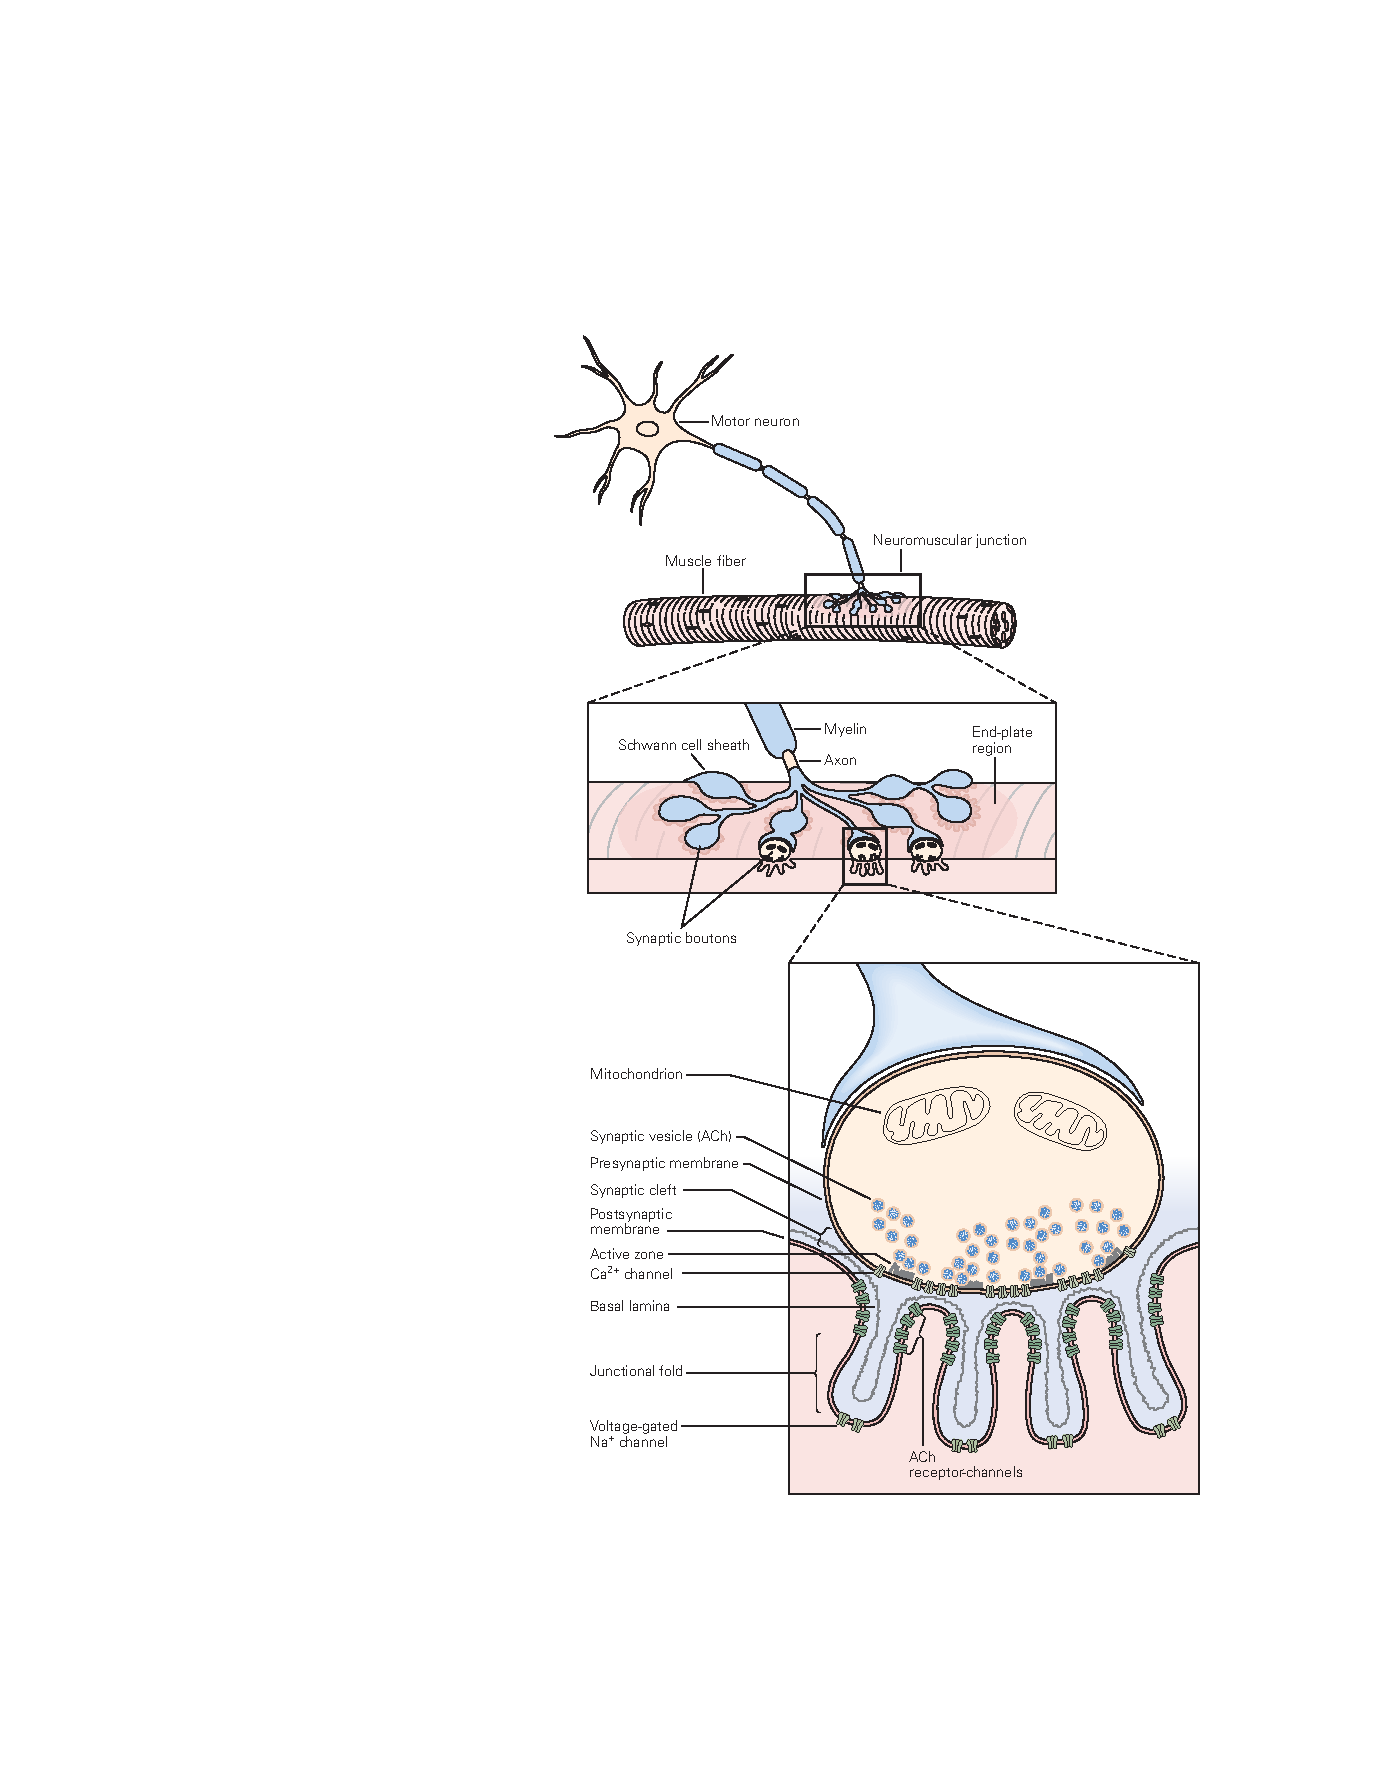
\includegraphics[width=0.75\linewidth]{chap12/fig_12_1}
	\caption{神经肌肉接头是研究化学突触信号的理想场所。
		在肌肉处,运动轴突分叉成几个约 2 μm 厚的细分支。
		每个分支形成多个肿块,称为突触环,上面覆盖着一层薄薄的\textit{施旺细胞}。
		结节接触肌纤维膜的一个特殊区域,即\textit{终板},并通过 100 nm 的\textit{突触间隙}与肌肉膜分开。
		每个结节都包含聚集在活跃区域周围的线粒体和突触小泡,神经递质\textit{乙酰胆碱}在这些区域被释放。
		紧接在终板每个环的下方是几个连接褶皱,其顶部含有高密度的\textit{乙酰胆碱}受体。
		肌肉纤维和神经末梢被一层结缔组织覆盖,基底层由胶原蛋白和糖蛋白组成。
		与细胞膜不同,基底层可自由渗透离子和小的有机化合物,包括\textit{乙酰胆碱}递质。
		突触前末端和肌纤维都将蛋白质分泌到基底层,包括乙酰胆碱酯酶,它通过将突触前末端释放的乙酰胆碱分解成醋酸盐和胆碱来使乙酰胆碱失活。
		基底层还通过将突触前环与突触后连接褶皱对齐来组织突触\cite{mcmahan1971visual}。}
	\label{fig:12_1}
\end{figure}


神经末梢位于肌肉表面的沟槽中,即初级褶皱中。
每个突触环下的膜进一步内陷形成一系列次级或连接褶皱(图~\ref{fig:12_1})。
神经末梢下方的肌肉细胞质包含许多可能参与突触特异性分子合成的圆形肌肉核。
它们不同于沿着肌纤维长度远离突触的扁平核。


轴突中的动作电位被传导到细分枝的末端,在那里它们触发\textit{乙酰胆碱}的释放。
突触结节包含合成和释放\textit{乙酰胆碱}所需的所有机制。
这包括含有递质\textit{乙酰胆碱}的突触小泡和突触小泡聚集的活动区。
此外,每个活动区都包含电压门控钙离子通道,这些通道通过每个动作电位将钙离子传导到末端。
钙离子的流入触发突触小泡与活性区质膜的融合,通过胞吐作用将突触小泡的内容物释放到突触间隙中(第~\ref{chap:chap15}~章)。


可以使用 $\alpha$-金环蛇毒素 ($\alpha$BTX) 研究\textit{乙酰胆碱}受体的分布,$\alpha$-金环蛇毒素($\alpha$BTX)是一种从\textit{银环蛇}的毒液中分离出来的肽,它与神经肌肉接头处的\textit{乙酰胆碱}受体紧密且特异地结合(图~\ref{fig:12_2}B)。 
碘化 BTX(125I-$\alpha$BTX)的定量放射自显影显示\textit{乙酰胆碱}受体堆积在次级褶皱的顶部,表面密度超过 $10,000/\mathrm{\mu m}^2$
(图~\ref{fig:12_3})。
负责定位受体的因素在第~\ref{chap:chap48}~章中讨论,我们将在其中考虑突触连接的发展。


\begin{figure}[htbp]
	\centering
	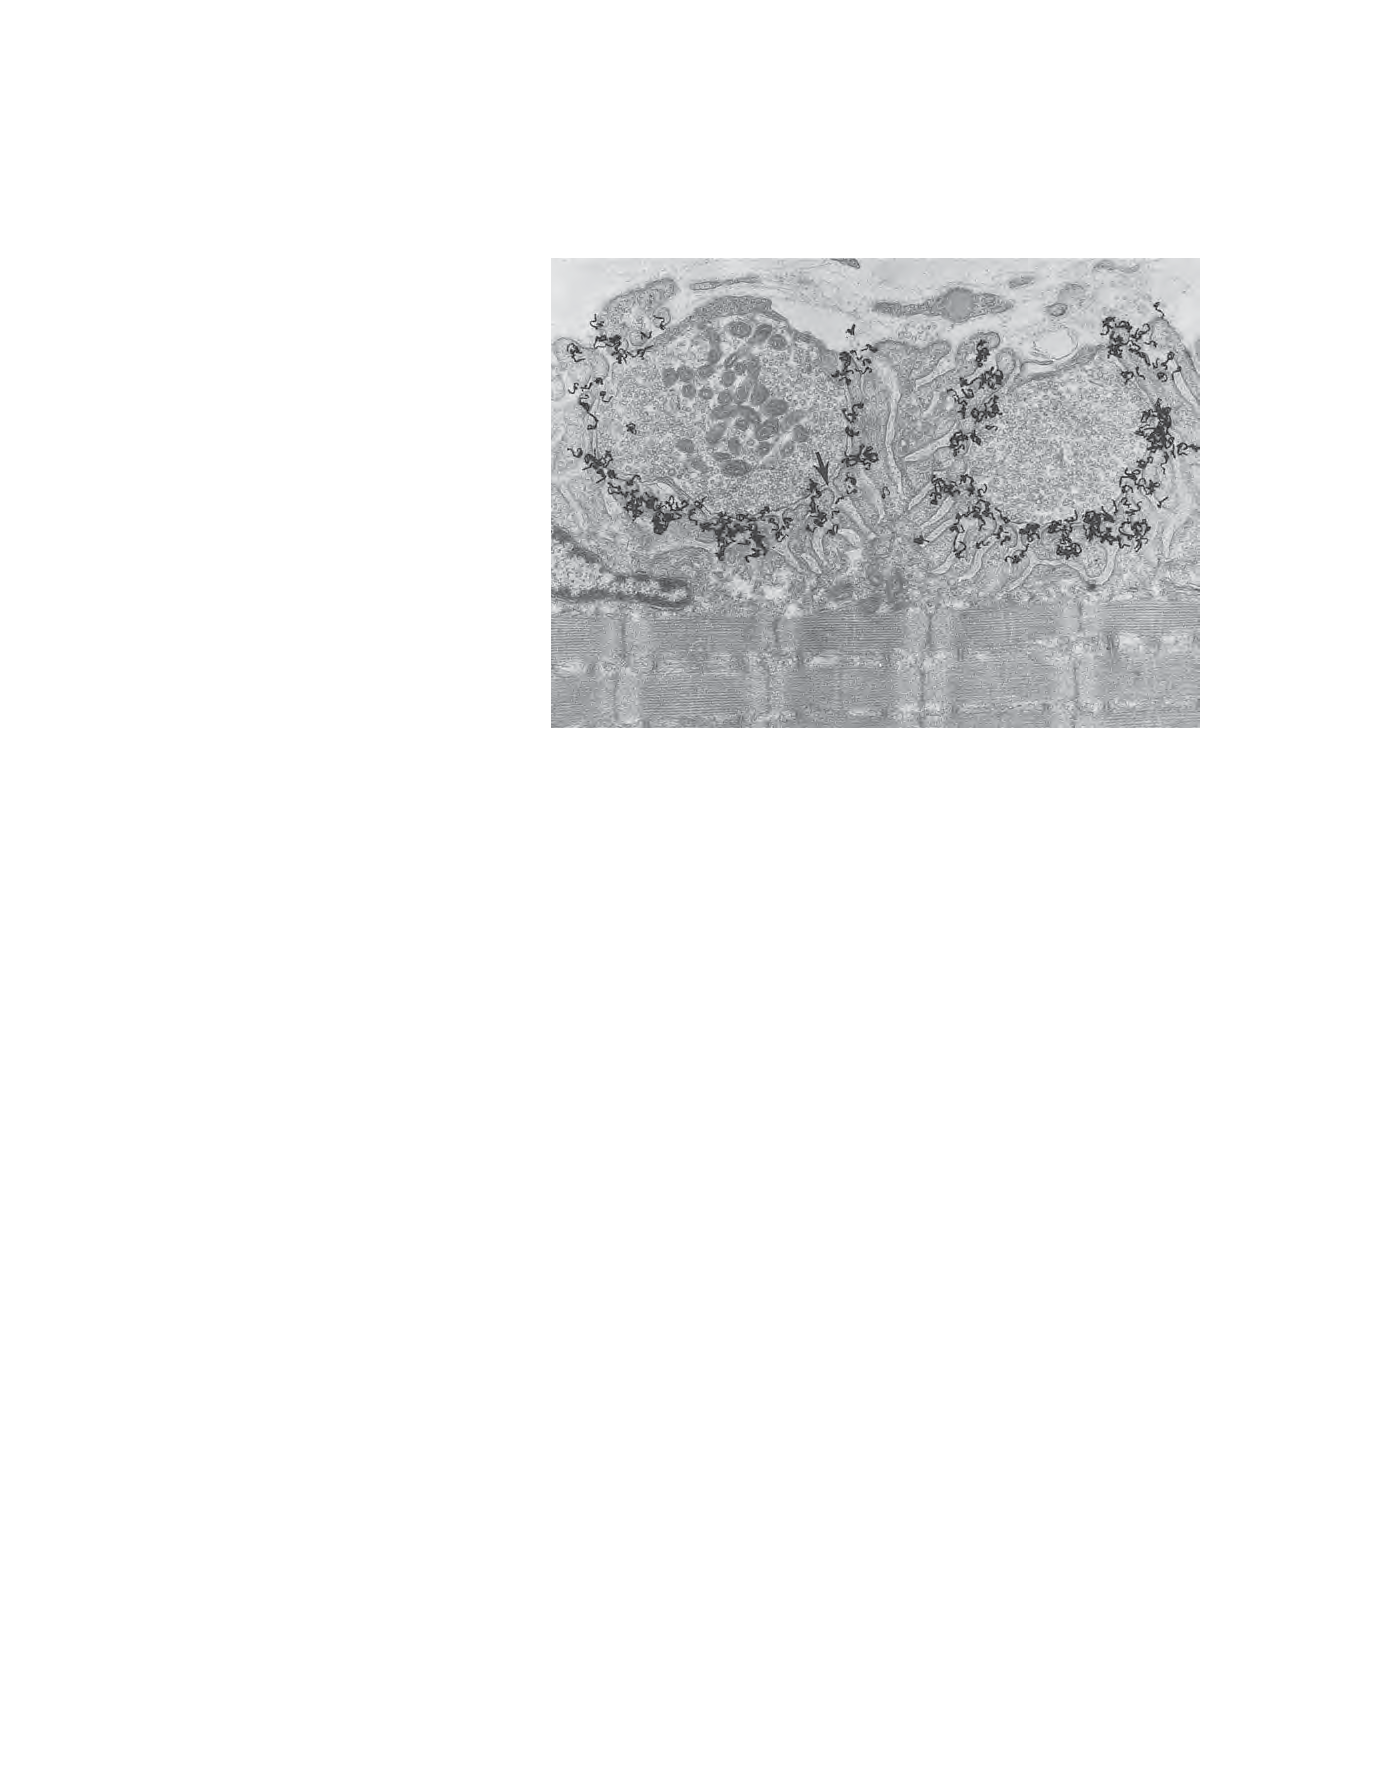
\includegraphics[width=0.75\linewidth]{chap12/fig_12_3}
	\caption{脊椎动物神经肌肉接头中的乙酰胆碱受体集中在连接褶皱的顶部三分之一处。
		这个富含受体的区域的特征是连接后膜的密度增加(箭头)。
		此处显示的放射自显影照片是通过首先将膜与放射性标记的$\alpha$-银环蛇毒素一起孵育而制成的,它与\textit{乙酰胆碱}受体结合。
		放射性衰变导致粒子发射,导致覆盖的银颗粒沿粒子轨迹叠加在一起(黑色颗粒)。
		放大倍率 ×18,000。}
	\label{fig:12_3}
\end{figure}



神经肌肉接头处的突触前膜和突触后膜被约 100 nm 宽的裂缝隔开。
尽管\textit{拉蒙-卡哈尔}在 19 世纪末提出了这样的差距,但直到 50 多年后用电子显微镜检查突触时才被可视化!
整个突触间隙都存在由胶原蛋白和其他细胞外基质蛋白组成的基底膜(基底层)。
\textit{乙酰胆碱酯酶}是一种快速水解\textit{乙酰胆碱}的酶,它被锚定在基底膜内的胶原纤维上。
释放到突触间隙中的\textit{乙酰胆碱}在到达肌肉膜中的\textit{乙酰胆碱}受体之前必须经过\textit{乙酰胆碱酯酶}的“挑战”。
由于\textit{乙酰胆碱酯酶}被高浓度\textit{乙酰胆碱}抑制,因此大多数分子都能通过。
然而,该酶将\textit{乙酰胆碱}的作用限制为“一次击中”,因为\textit{乙酰胆碱酯酶}一旦与突触后膜中的受体分离,就会水解递质。



\subsection{膜通透性的局部变化导致突触后电位变化}

一旦\textit{乙酰胆碱}从突触末端释放,它会迅速结合并打开终板膜中的\textit{乙酰胆碱}受体通道。
这导致肌肉膜对阳离子的渗透性显著增加,导致正电荷进入肌肉纤维并使终板膜快速去极化。
由此产生的\textit{兴奋性突触后电位}非常大;
单个运动轴突的刺激产生大约 75 毫伏 的\textit{兴奋性突触后电位}。
在神经肌肉突触处,\textit{兴奋性突触后电位}也称为终板电位。


膜电位的这种变化通常大到足以快速激活肌肉膜中的电压门控 \ce{Na+} 通道,将终板电位转化为动作电位,然后沿肌纤维传播。
由于连接褶皱底部的电压门控 \ce{Na+} 通道密度很高,终板在肌肉中产生动作电位的阈值特别低。
一个非常大的\textit{兴奋性突触后电位}和低阈值的组合,使触发肌纤维动作电位的安全系数非常高。
相反,在中枢神经系统中,大多数突触前神经元产生的突触后电位幅度小于 1 mV ,因此需要来自多个突触前神经元的输入才能在大多数中枢神经元中产生动作电位。


\textit{保罗$\cdot$法特}和\textit{伯纳德$\cdot$卡茨}在 1950 年代首先使用细胞内电压记录详细研究了终板电位。
\textit{法特}和\textit{卡茨}能够通过应用箭毒药物(图~\ref{fig:12_2}A)来降低突触后电位的幅度,以其振幅低于动作电位的阈值,从而能够分离出终板电位(图~\ref{fig:12_4})。
在终板,突触电位在 1 到 2 毫秒内上升,但衰减得更慢。
通过在肌肉纤维的不同点进行记录,\textit{法特}和\textit{卡茨}发现\textit{兴奋性突触后电位}在终板处最大,并随着距离的增加而逐渐减小(图~\ref{fig:12_5})。
此外,\textit{兴奋性突触后电位}的时间进程随着距离的增加而逐渐减慢。


\begin{figure}[htbp]
	\centering
	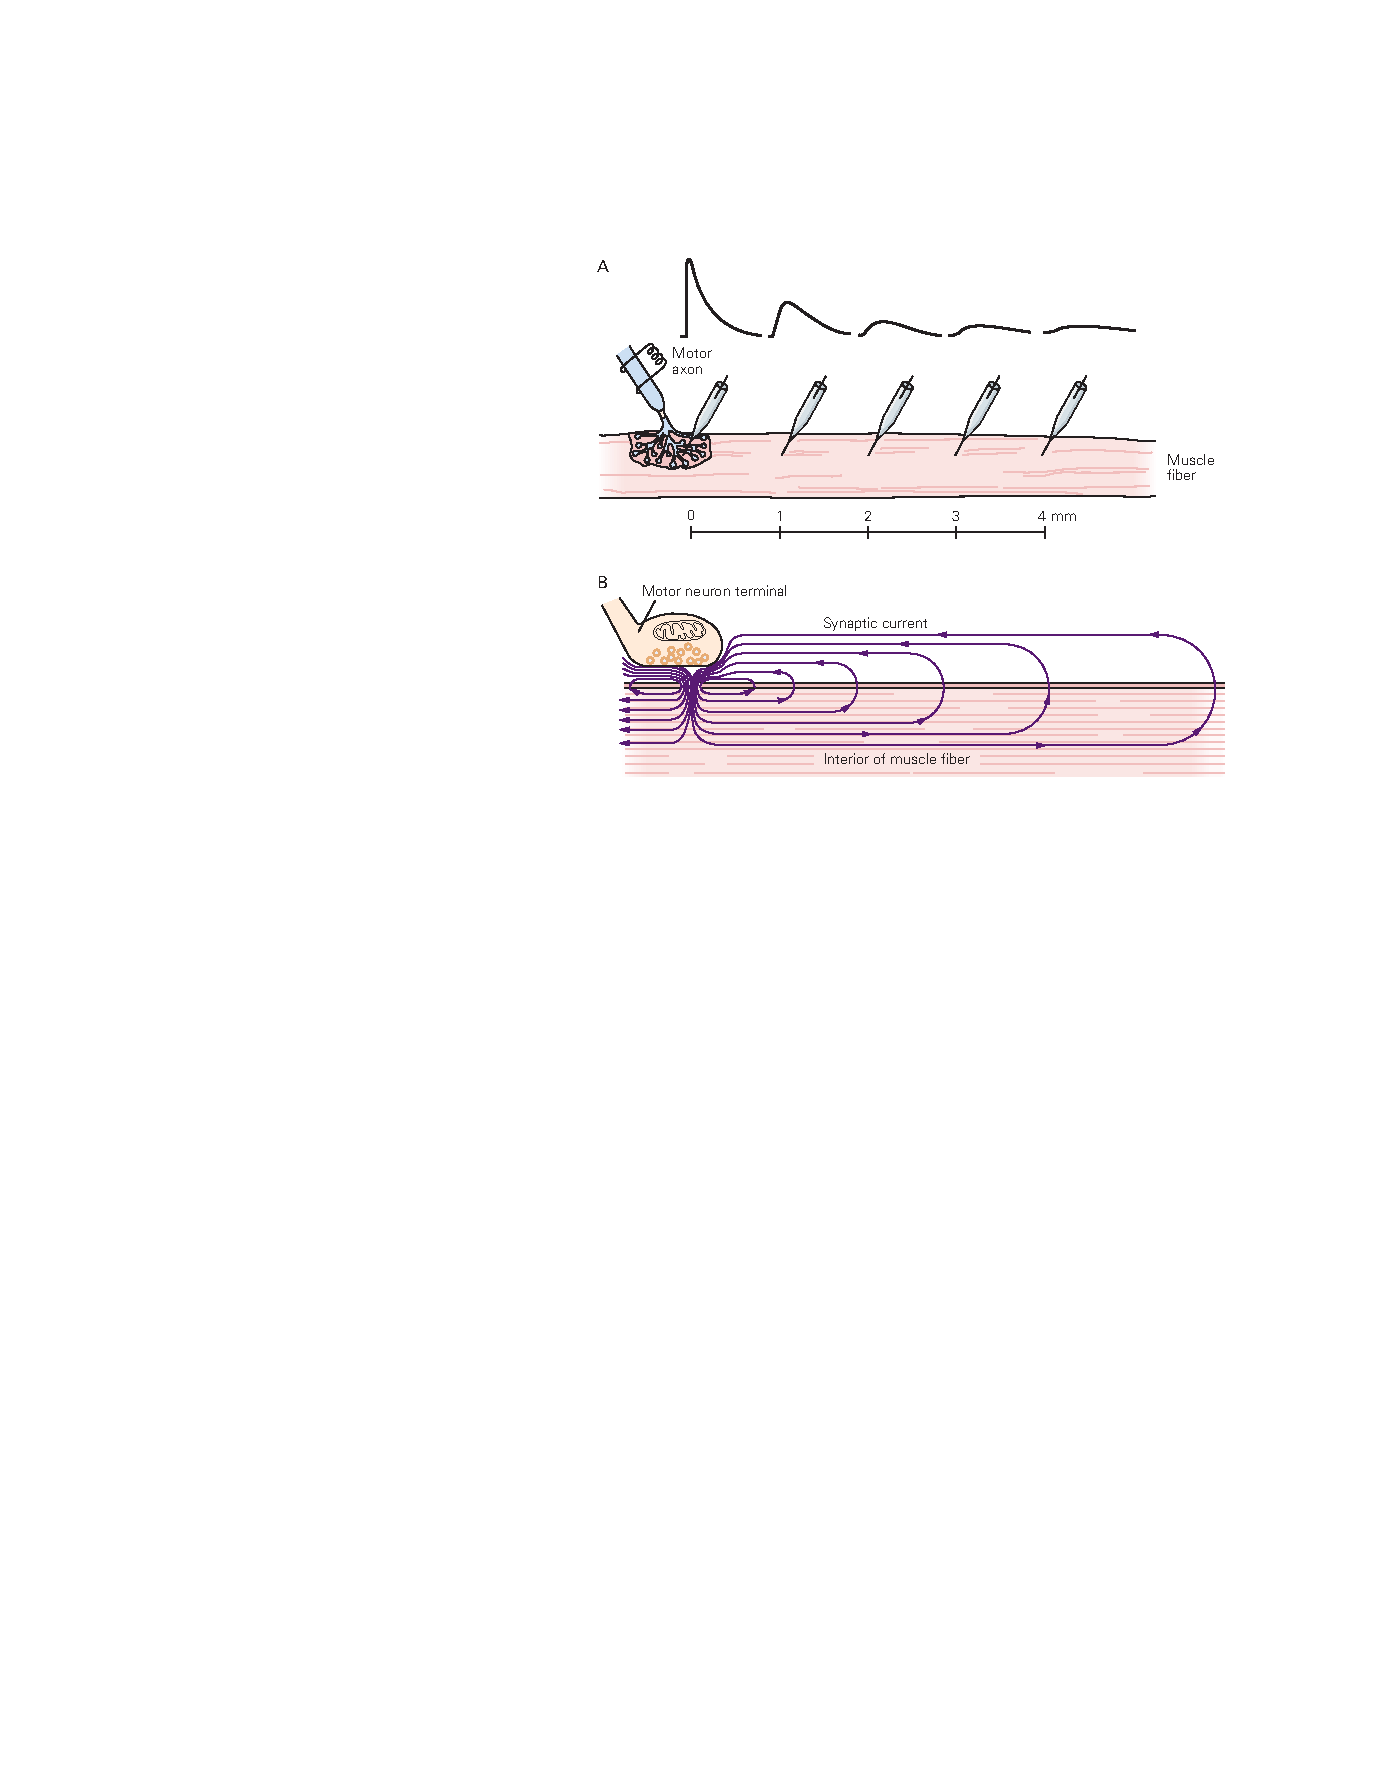
\includegraphics[width=0.8\linewidth]{chap12/fig_12_5}
	\caption{终板电势随着它被动的从终板处传播开去,振幅随距离减少。
		\textbf{A.} 突触后电位的振幅减小,并且电位的时间进程随距离离开起始点而减慢。
		\textbf{B.} 这种衰减是由于肌肉纤维膜的泄漏导致的。
		因为电荷必须在一个完整的回路中流动,所以终板处的内向突触电流会通过静息通道和脂质双层( 即电容器)产生返回的外向电流。 
		这种返回的正电荷向外流动使膜去极化。 
		因为电流沿着膜一直漏出,所以向外的电流和由此产生的去极化会随着与终板的距离的增加而减小。}
	\label{fig:12_5}
\end{figure}


\begin{figure}[htbp]
	\centering
	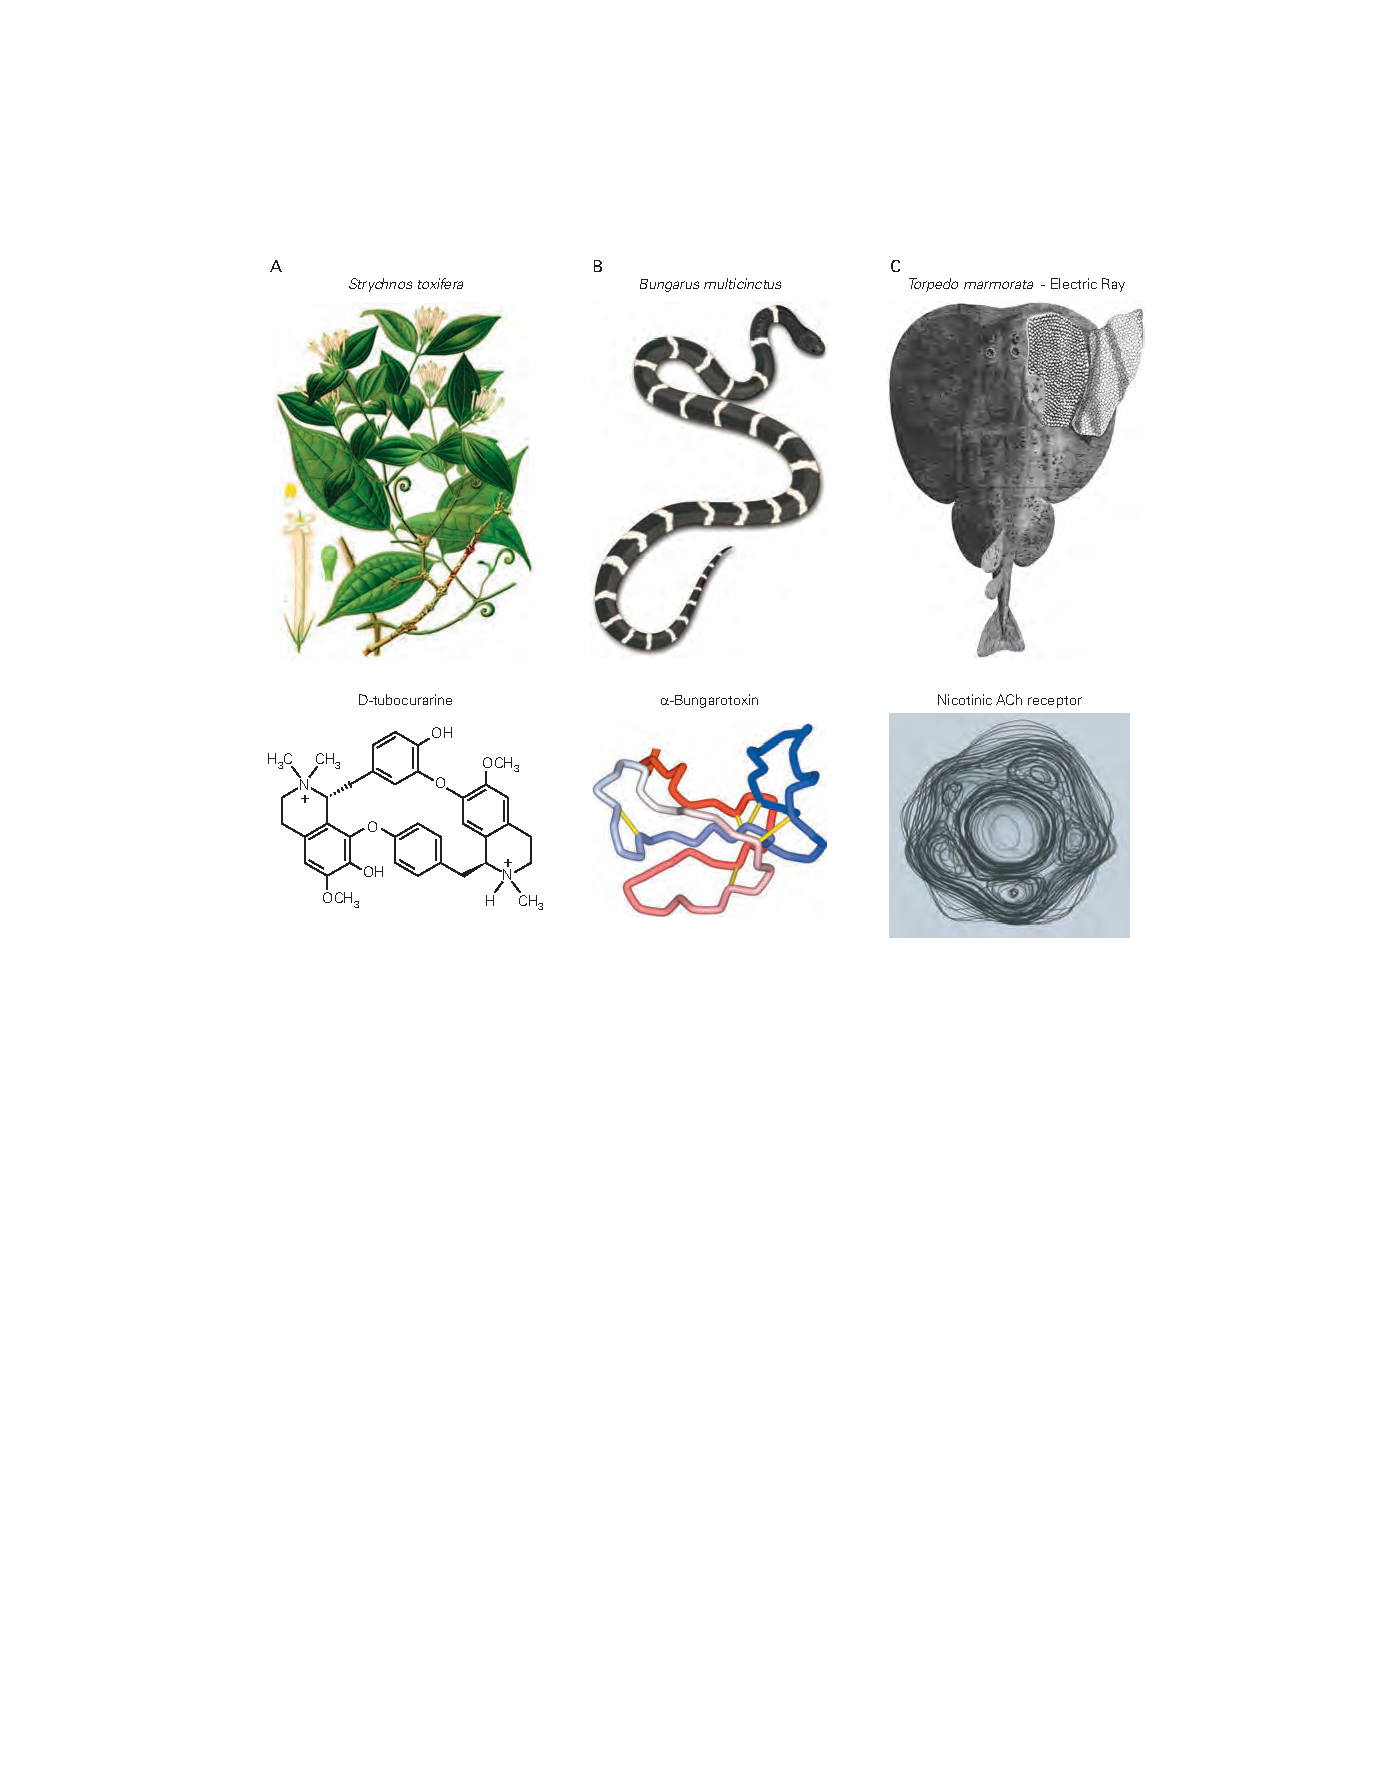
\includegraphics[width=1.0\linewidth]{chap12/fig_12_2}
	\caption{毒药、毒液和高压电鱼有助于阐明烟碱乙酰胆碱受体的结构和功能。 
	\textbf{A}:箭毒是从马钱子的叶子中提取的毒素混合物,南美土著人涂在箭头上来麻痹他们的猎物。
	活性化合物 \textit{D-筒箭毒碱}是一种复杂的多环结构化合物,带有带正电荷的胺基,与\textit{乙酰胆碱}有一些相似之处。
	它与烟碱受体上的\textit{乙酰胆碱}结合位点紧密结合,作为\textit{乙酰胆碱}的竞争性拮抗剂发挥作用。
	\textbf{B}$\alpha$-金环蛇毒素是从金环蛇(B ungarus)的毒液中提取的。
	它是一种包含 5 个二硫键(黄线)的 74 氨基酸多肽,产生了刚性结构。
	该毒素与\textit{乙酰胆碱}结合位点极其紧密地结合,并作为\textit{乙酰胆碱}的不可逆、非竞争性拮抗剂发挥作用。
	\textbf{C}. \textit{石纹电鳐}有一个特殊的结构,即电器官,它由大量小而扁平的肌肉状细胞或电斑组成,像电池堆一样串联排列。
	当运动神经释放\textit{乙酰胆碱}时,大量烟碱\textit{乙酰胆碱}受体通道的打开会产生大电流,从而在鱼体外产生高达 200 伏特的非常大的电压降,使附近的猎物昏迷。
	电板为\textit{乙酰胆碱}受体的生化纯化和表征提供了丰富的来源。}
	\label{fig:12_2}
\end{figure}


\begin{figure}[htbp]
	\centering
	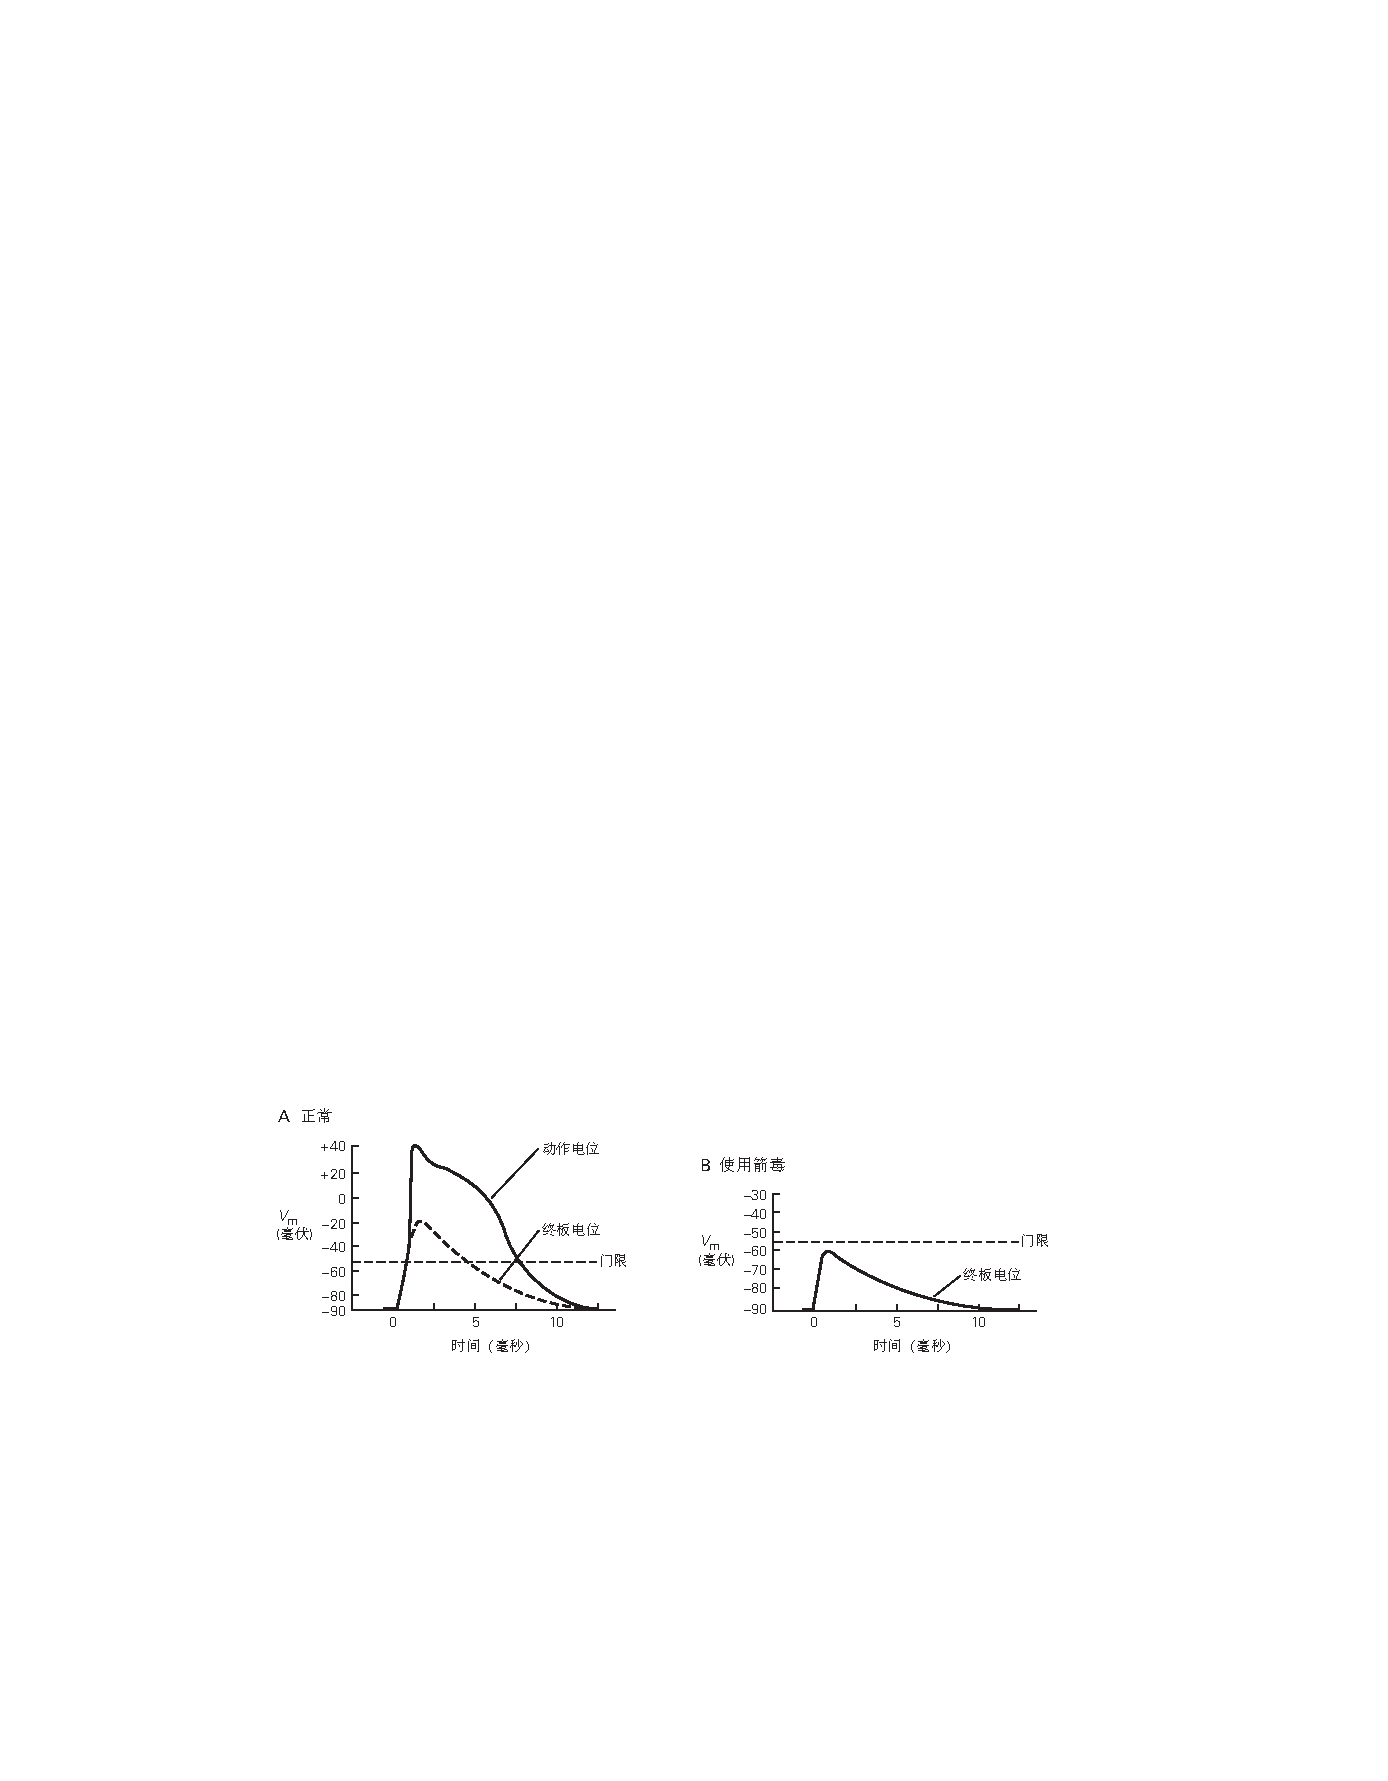
\includegraphics[width=1.0\linewidth]{chap12/fig_12_4}
	\caption{终板电位可以通过药理学方法单独分离出来进行研究。
		\textbf{A.} 在正常情况下,运动轴突的刺激会在骨骼肌细胞中产生一个动作电位。
		图中的虚线曲线显示了触发动作电位的终板电位的推断时间轨迹。
		较浅的虚线表示动作电位的阈值。
		\textbf{B.} 箭毒阻断\textit{乙酰胆碱}与其受体的结合,从而防止终板电位达到动作电位的阈值。
		通过这种方式,有助于研究产生终板电位的电流和通道,这与产生动作电位的电流和通道不同。
		此处显示的终板电位是在存在低浓度箭毒的情况下记录的,该浓度下箭毒仅阻断一部分\textit{乙酰胆碱}受体。
		这些细胞内记录中的静息电位(–90  mV )、终板电位和动作电位值是脊椎动物骨骼肌的特征。}
	\label{fig:12_4}
\end{figure}


由此,\textit{法特}和\textit{卡茨}得出结论,终板电位是由局限在终板的内向离子电流产生的,然后这种电流被动地扩散开来。
( 内向电流对应于正电荷的流入,使膜内部去极化。)内向电流被限制在终板,是因为\textit{乙酰胆碱}受体集中在那里,与释放递质的突触前末端相对应。
作为距离的增加,\textit{兴奋性突触后电位}振幅减小和速度减慢是肌肉纤维的被动电缆特性的结果。


\textit{斯蒂芬$\cdot$库夫勒}及其同事他们使用一种称为微离子电渗疗法的技术将\textit{乙酰胆碱}应用于肌肉膜上的精确点,提供了表明\textit{乙酰胆碱}受体局限于终板的电生理学证据。
在这种方法中,通过向电极内部施加正电压,带正电荷的乙酰胆碱从充满乙酰胆碱的细胞外微电极中排出。
将终板区域暴露于蛋白水解酶可使神经末梢从肌肉表面拉开,并将\textit{乙酰胆碱}直接应用于小微电极尖端正下方的突触后膜。
使用这种技术,\textit{库夫勒}发现在突触末端几微米内,对\textit{乙酰胆碱}的突触后去极化反应急剧下降。


电压钳实验表明,终板电流的上升和衰减比由此产生的终板电势更快(图~\ref{fig:12_6})。
终板电流的时间过程直接由\textit{乙酰胆碱}受体通道的快速打开和关闭决定。
因为离子电流对肌肉膜电容充电或放电需要时间,从而改变膜电压,所以\textit{兴奋性突触后电位}滞后于突触电流(参见图~\ref{fig:9_10}~和本章末尾的附言)。


\begin{figure}[htbp]
	\centering
	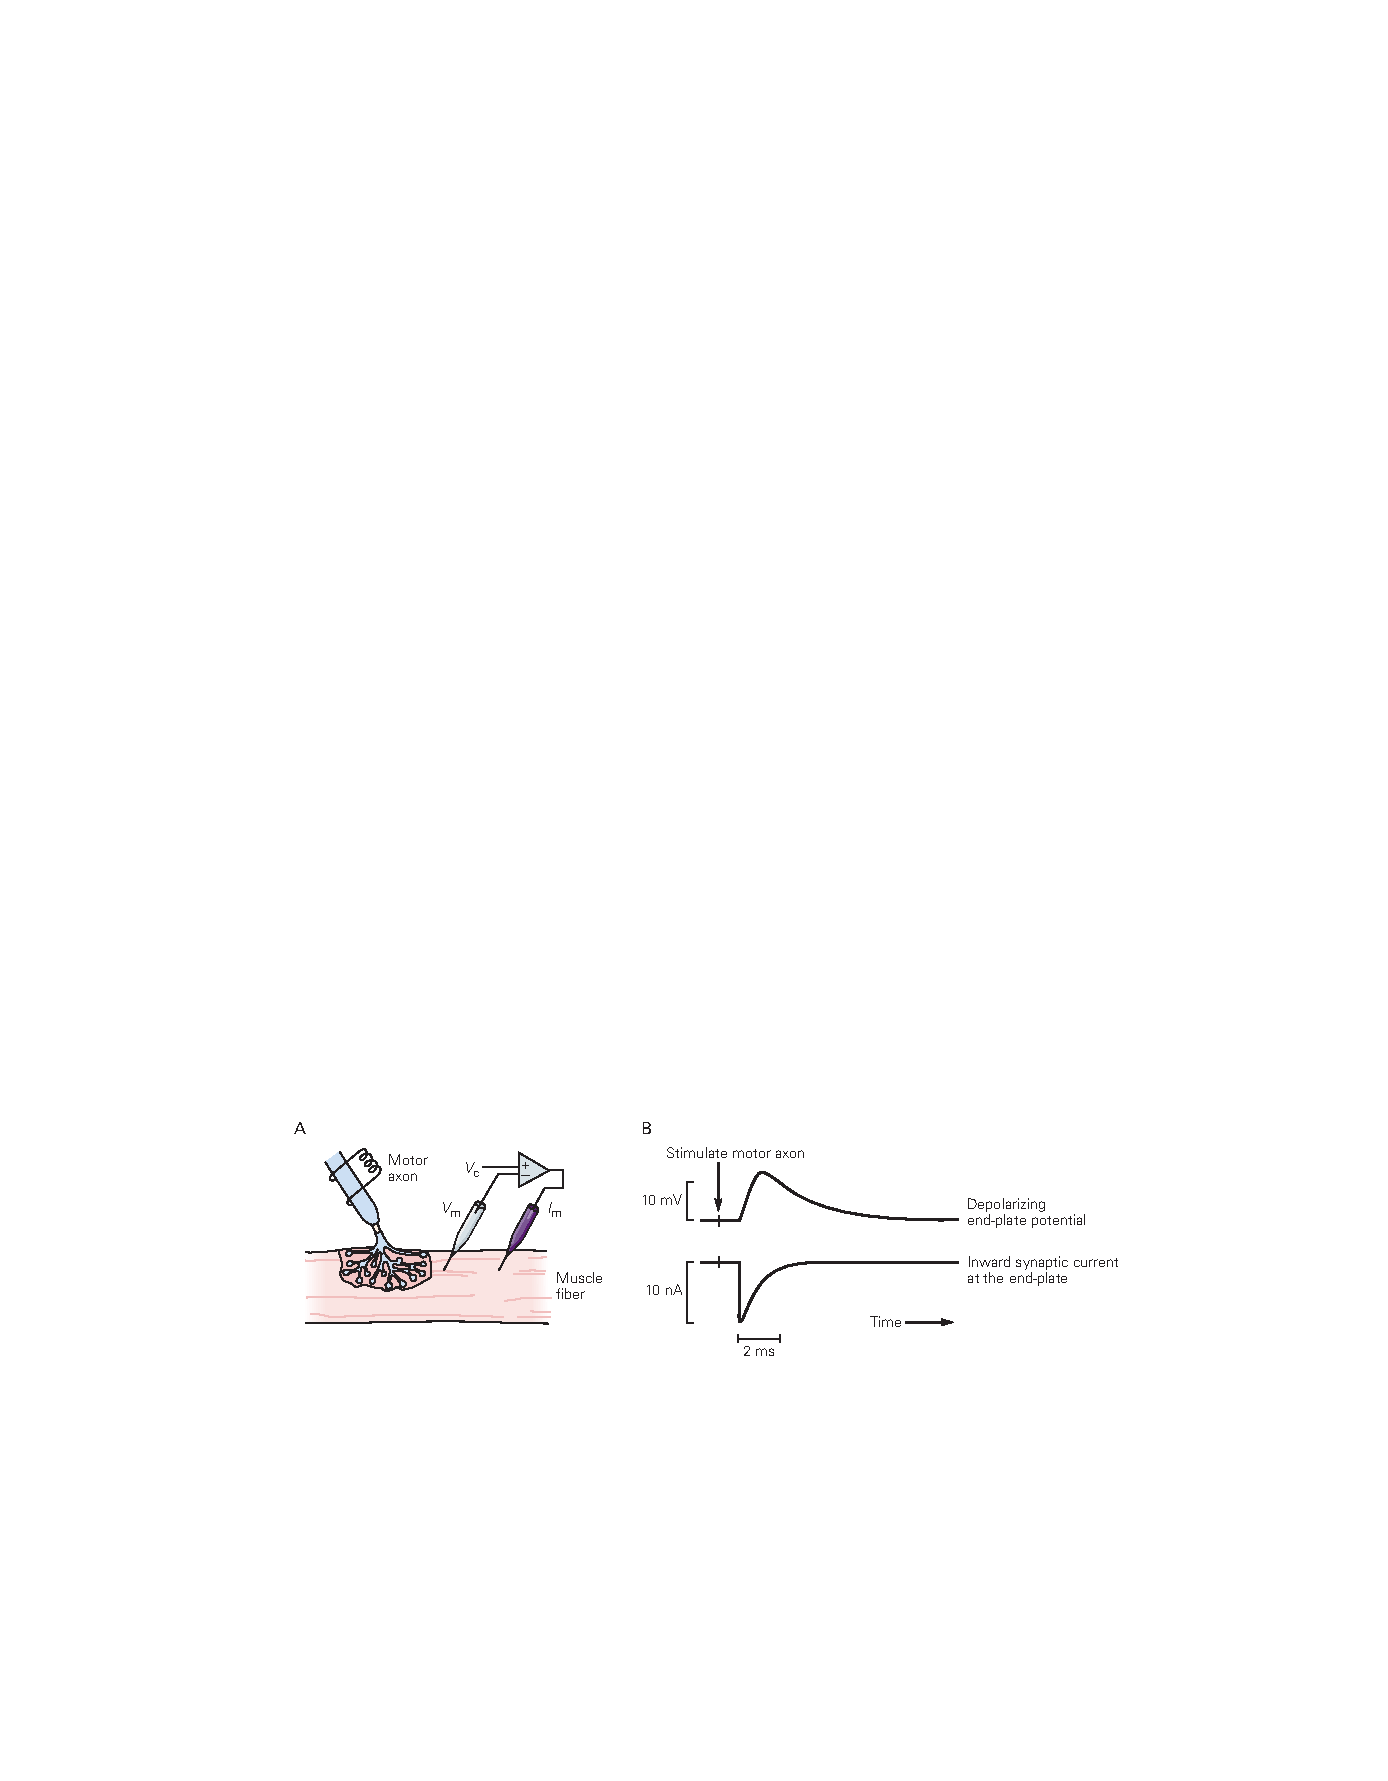
\includegraphics[width=1.0\linewidth]{chap12/fig_12_6}
	\caption{终板电流比终板电势增加和衰减得更快。
		\textbf{A.} 通过将两个微电极插入终板附近的肌肉中,对终板处的膜进行电压钳制。
		一个电极测量膜电位($V_m$),第二个电极测量电流($I_m$)。
		两个电极都连接到负反馈放大器,以确保输送足够的电流($I_m$),以便$V_m$保持钳位在命令电位 $V_c$处。
		然后可以在恒定 $V_m$ 下测量通过刺激运动神经引发的突触电流,例如 -90 mV (见方框~\ref{box:10_1})。
		\textbf{B.} 终板电位(在 $V_m$ 未被钳制时测得)变化相对缓慢,滞后于更快速的内向突触电流( 在电压钳制条件下测得)。
		这是因为在肌肉膜去极化之前,突触电流必须首先改变肌肉膜电容上的电荷,然后肌肉膜才能去极化。}
	\label{fig:12_6}
\end{figure}



\subsection{神经递质乙酰胆碱以离散包的形式释放}

\textit{法特}和\textit{卡茨}在 1950 年代首次在青蛙运动终板进行微电极记录时,观察到小的自发去极化电位(0.5–1.0 mV ),平均速率约为 1/s。 
这种自发电位仅限于终板区域,与刺激诱发的\textit{兴奋性突触后电位}表现出相同的时间过程,并被箭毒阻断。 
因此,它们被命名为\textit{微终板电位}。


什么可以解释微型终板电位的小而固定的尺寸? 
\textit{德尔$\cdot$卡斯蒂略}和\textit{卡茨}测试了\textit{微兴奋性突触后电位}代表单个\textit{乙酰胆碱}分子作用的可能性。
这个假设很快就被否定了,因为将非常少量的\textit{乙酰胆碱}应用于终板可以引起远小于 1.0-mV\textit{微兴奋性突触后电位}的去极化反应。 
低剂量的\textit{乙酰胆碱}确实会增加基线波动或“噪音”。 
后来对该噪声的统计成分的分析表明,潜在的单一突触后反应是振幅为 0.3 微伏且持续时间为 1.0 毫秒的去极化。 
这是单个\textit{乙酰胆碱}受体通道(稍后描述)的电信号特性的第一个提示线索。


\textit{德尔$\cdot$卡斯蒂略}和\textit{卡茨}得出结论,每个\textit{微兴奋性突触后电位}必须代表多分子包或“量子”递质的作用。 
此外,他们认为由刺激诱发的大型\textit{兴奋性突触后电位}由整数个量子组成。 
第~\ref{chap:chap15}~章介绍了该量子假说的证据。



\section{单个乙酰胆碱受体通道传导全有或无电流}

产生产生去极化终板电位的内向电流的\textit{乙酰胆碱}受体通道的特性是什么?
哪些离子通过通道移动以产生这种内向电流?
单个\textit{乙酰胆碱}受体通道携带的电流是什么样的?


1976 年,\textit{厄温$\cdot$内尔}和\textit{伯特$\cdot$萨克曼}从骨骼肌细胞中单个\textit{乙酰胆碱}受体通道传导的电流记录中获得了对\textit{乙酰胆碱}受体通道功能的生物物理性质的重要见解,即单一电流或基本电流。
他们发现,打开单个通道会产生非常小的矩形离子电流脉冲(图~\ref{fig:12_7}A)。
在给定的静息电位下,每个通道开口都会产生相同大小的电流脉冲。
在 −90 mV 时,电流阶跃的振幅约为 −2.7 皮安。 
虽然这是一个非常小的电流,但它相当于每秒约 1700 万个离子的流动!


\begin{figure}[htbp]
	\centering
	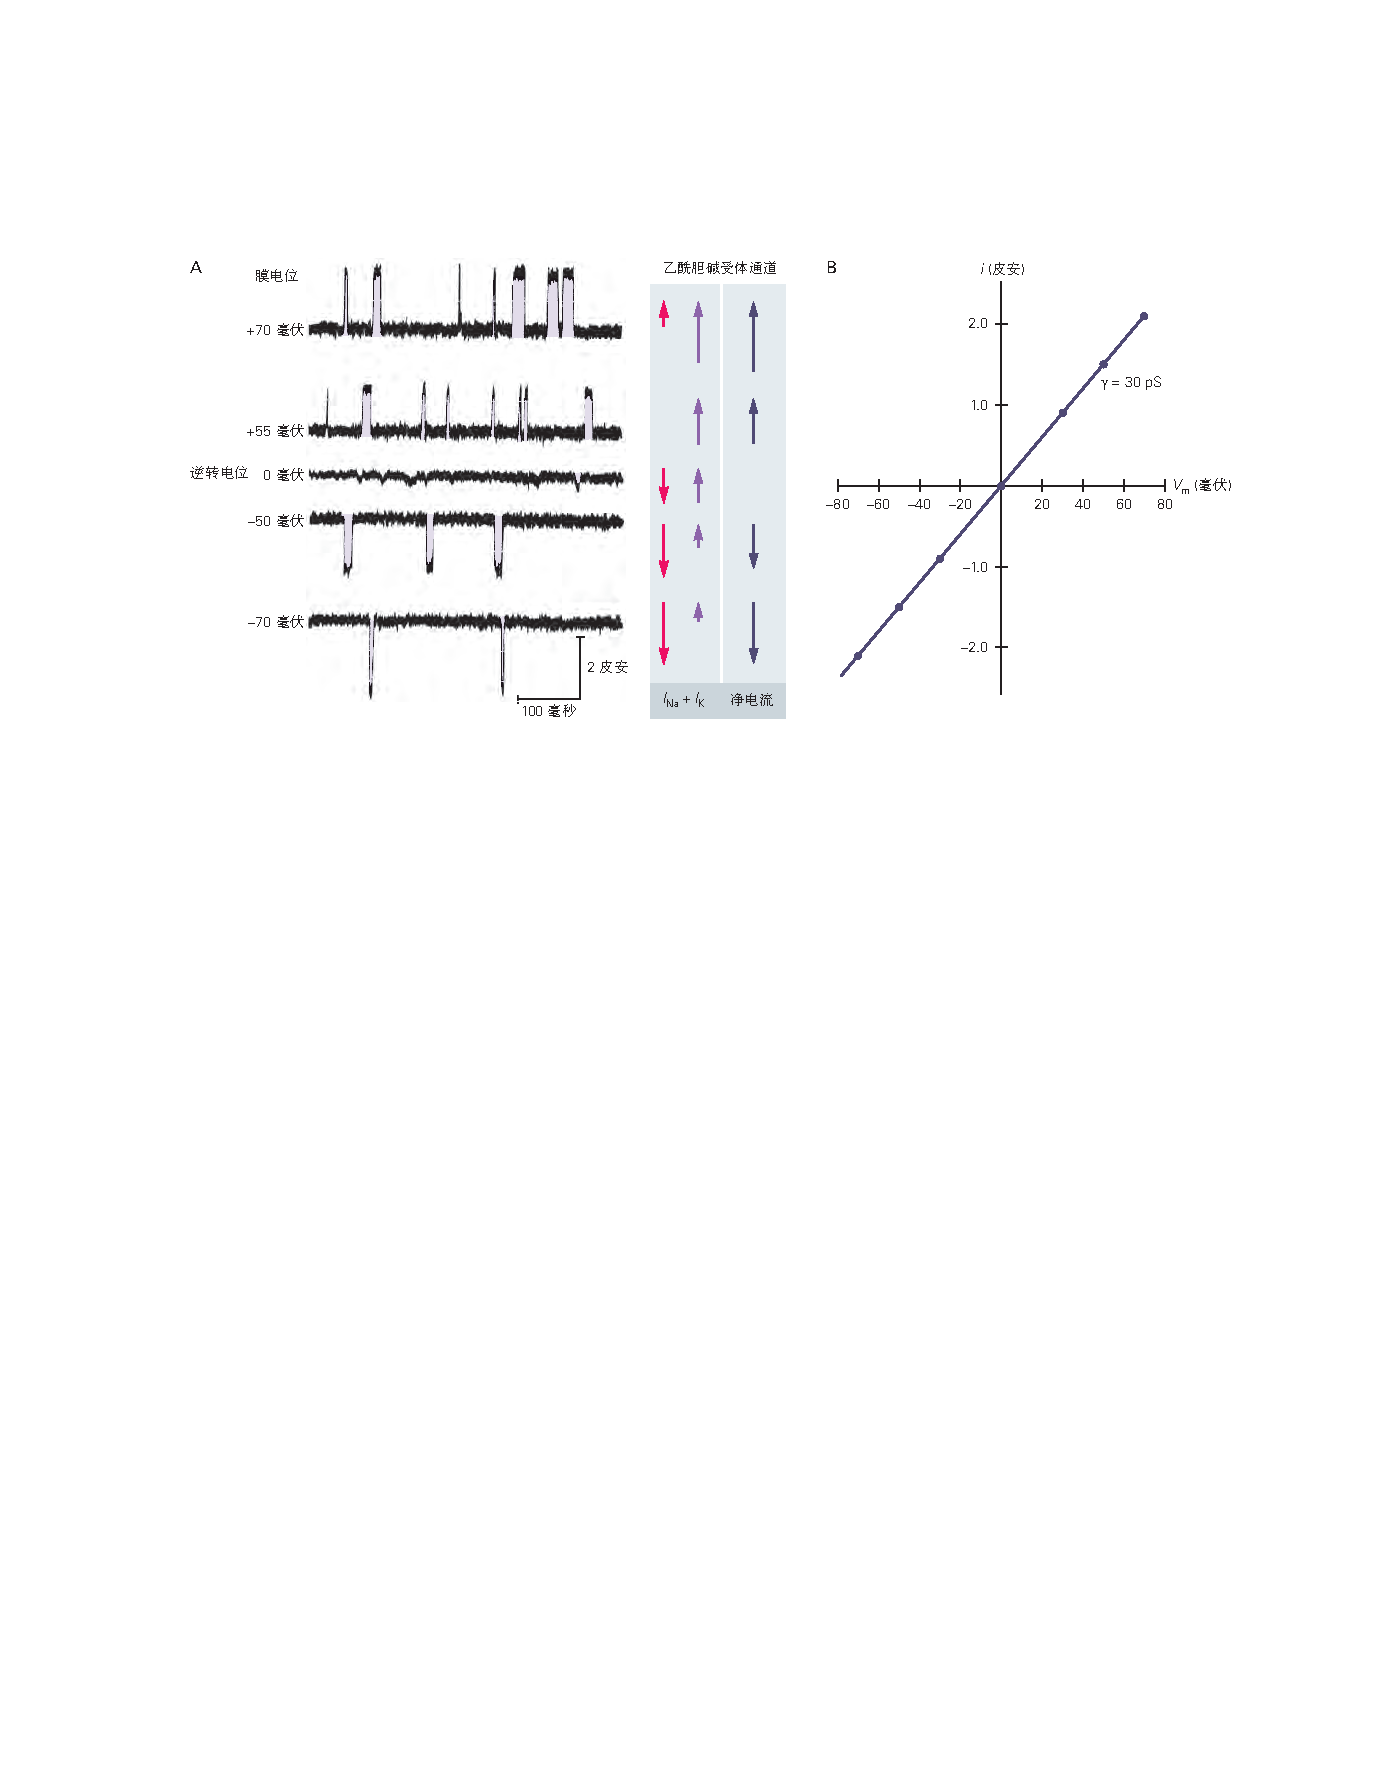
\includegraphics[width=1.0\linewidth]{chap12/fig_12_7}
	\caption{单个\textit{乙酰胆碱}受体通道传导全有或全无的基本电流。
		\textbf{A.} 膜片钳技术用于记录单个\textit{乙酰胆碱}受体通道的电流。
		贴片电极充满含有低浓度\textit{乙酰胆碱}的盐溶液,然后与肌肉膜表面紧密接触(见方框~\ref{box:8_1})。
		在固定的膜电位下,每次通道打开时,它都会产生相对恒定的基本电流。
		在 –90 mV 的静息电位下,电流约为 −2.7 皮安(1 皮安 = $10^{-12}$安)。
		随着膜片上的电压系统地变化,合成电流的幅度会因驱动力的变化而变化。
		电流在负电压至 0 mV 时向内,在正电压至 0 mV 时向外,因此将 0 mV 定义为反转电位。
		迹线右侧的箭头说明了单独的钠和钾通量以及作为电压函数的合成净电流。
		\textbf{B.} 通过单个\textit{乙酰胆碱}受体通道的电流与膜电压之间的线性关系表明,该通道表现为一个简单的电阻器,其单通道电导(f)约为 30 pS。}
	\label{fig:12_7}
\end{figure}



\subsection{终板的离子通道可渗透钠离子和钾离子}

虽然通过单个\textit{乙酰胆碱}受体通道的电流幅度对于每次打开都是恒定的,但每次打开的持续时间和打开之间的时间差异很大。
这些变化是因为通道的打开和关闭,是随机的;
它们遵循描述放射性衰变指数时间过程的相同统计规律。 
由于通道和\textit{乙酰胆碱}会经历随机的热运动和波动,因此无法准确预测任何一个通道结合\textit{乙酰胆碱}需要多长时间,或者在\textit{乙酰胆碱}解离和通道关闭之前该通道将保持打开状态多长时间。
然而,特定类型通道保持打开的平均时间长度是该通道的明确定义的属性,就像放射性衰变的半衰期是特定同位素的不变属性一样。
\textit{乙酰胆碱}受体通道的平均开放时间约为 1 ms 。
因此,每个通道开口允许大约 17000 个离子移动。
一旦通道关闭,\textit{乙酰胆碱}分子就会解离,通道保持关闭状态,直到它再次与\textit{乙酰胆碱}结合。


一旦受体通道打开,哪些离子会流过通道,这如何导致肌肉膜去极化?
识别负责突触电流的离子( 或多个离子)的一种重要方法是测量推动离子通过通道的化学驱动力( 化学电池)的值。
请记住,通过单个开放通道的电流由单通道电导率与通过通道传导的离子的电化学驱动力的乘积给出(第~\ref{chap:chap9}~章)。 
因此,单个\textit{乙酰胆碱}受体通道产生的电流由下式给出:


\begin{equation}
	I_{\text{EPSP}} = \gamma_{\text{EPSP}}\times (V_m - E_{\text{EPSP}}),
\end{equation}


其中 $I_{\text{EPSP}}$ 是通过一个通道的电流幅度,$\gamma_{\text{EPSP}}$ 是单个开放通道的电导,$ E_{\text{EPSP}} $ 是膜电位,此时通过通道的离子净通量为零,$V_m - E_{\text{EPSP}}$ 是离子通量的电化学驱动力。
由于驱动力的变化,电流步长随着膜电位的变化而变化。 
对于\textit{乙酰胆碱}受体通道,$I_{\text{EPSP}}$与膜电压呈线性关系,表明单通道电导是恒定的,不依赖于膜电压;
也就是说,通道表现为一个简单的欧姆电阻。
根据该关系的斜率,发现通道的电导为 30 pS(图~\ref{fig:12_7}B)。
正如我们在第~\ref{chap:chap9}~章中看到的,由于许多受体通道(n)的开放,总电导 g 由下式给出:


\begin{equation}
	g = n \times \gamma.
\end{equation}


单个通道的电流-电压关系表明,通过\textit{乙酰胆碱}受体通道的离子电流的反转电位( 从膜电压轴的截距获得)为 0 mV ,这不等于 \ce{Na+} 其他主要阳离子或阴离子任何的平衡电位 。
这是因为这种化学势不是由单一离子种类产生,而是由两种离子种类的组合产生:终板上的配体门控通道几乎对两种主要阳离子 \ce{Na+} 和 \ce{K+} 具有同等的渗透性。
因此,在终板电位期间,\ce{Na+} 流入细胞,\ce{K+} 流出。
反转电位为 0 mV,因为这是 \ce{Na+} 和 \ce{K+} 平衡电位的加权平均值(方框~\ref{box:12_1})。
在反转电位处,\ce{Na+} 的流入被 \ce{K+} 的等量流出所平衡(图~\ref{fig:12_7}A)。


\begin{proposition}[终板电位的反转电位] \label{box:12_1}
	
	\quad \quad 由一种以上离子物种携带的膜电流的反转电位,例如通过\textit{乙酰胆碱}受体通道的终板电流,由两个因素决定:
	(1) 渗透离子的相对电导( 在终板电流的情况下为$g_{Na}$和$g_K$)和(2)离子的平衡电位($E_{Na}$和$E_K$)。
	
	\quad \quad 在\textit{乙酰胆碱}受体通道电流的反转电位下,\ce{Na+}携带的内向电流与\ce{K+}携带的外向电流平衡:
	
	\begin{equation}\label{eq:12_inward_current}
		I_{Na} + I_K = 0.
	\end{equation}
	
	\quad \quad 单个\ce{Na+}和\ce{K+}电流可以从以下两个方程获得:
	\begin{equation}\label{eq:12_Na_current}
		I_{Na} = g_{Na} \times (V_m - E_{Na})
	\end{equation}

	\begin{equation}\label{eq:12_K_current}
		I_K = g_K \times (V_m - E_K).
	\end{equation}
	
	\quad \quad 我们可以用等式~\ref{eq:12_inward_current}~中的$ I_{Na} $和$ I_K $替换等式~\ref{eq:12_Na_current}~和~\ref{eq:12_K_current},用$E_{\text{EPSP}}$替换$V_m$(因为在反转电位$V_m = E_{\text{EPSP}}$时):
	\begin{equation}\label{eq:12_substitude_inward_current}
		g_{Na} \times (E_{\text{EPSP}} - E_{Na}) + 
		g_K \times (E_{\text{EPSP}} - E_K)
		= 0.
	\end{equation}
	
	\quad \quad 求解$ E_{\text{EPSP}} $的这个方程生成:
	\begin{equation}\label{eq:12_solving_EPSP}
		E_{\text{EPSP}} = 
			\frac{
				g_{Na} \times E_{Na} + (g_K \times E_K)
			}
			{
				g_{Na} + g_K
			}.
	\end{equation}
	
	\quad \quad 如果知道$E_{\text{EPSP}}$、$E_K$和$E_{Na}$,该方程也可用于求解$g_{Na} / g_K$/比。
	因此,重新排列方程式~\ref{eq:12_solving_EPSP}~产生:
	\begin{equation}\label{eq:12:rearranging_EPSP}
		\frac{g_{Na}}{g_K} = 
		\frac{E_{\text{EPSP}} - E_{K}}{E_{Na} - E_{\text{EPSP}}}.
	\end{equation}
	
	\quad \quad 在神经肌肉接头处,$E_{\text{EPSP}}$=0 毫伏,$E_K$=-100 毫伏,$E_{Na}$=+55 毫伏。
	因此,从等式~\ref{eq:12:rearranging_EPSP}~可以看出,$g_{Na} / g_K$的值约为1.8,表明\textit{乙酰胆碱}受体通道对\ce{Na+}的电导略高于对\ce{K+}的电导。
	一种可比较的方法可用于分析中枢神经元兴奋性和抑制性突触电位期间的反转电位和离子运动(第~\ref{chap:chap13}~章)。
	
\end{proposition}



终板上的\textit{乙酰胆碱}受体通道对单一离子种类没有选择性,电压门控的 \ce{Na+} 或 \ce{K+} 通道也是如此,因为\textit{乙酰胆碱}受体通道的孔径远大于电压门控孔径-门控通道。
电生理测量表明它的直径可能为 0.6 nm ,这是根据可以渗透通道的最大有机阳离子的大小进行的估计的。
例如,\textit{四甲胺}的直径约为 0.6 nm,但仍会渗透到通道中。
相比之下,电压门控 \ce{Na+} 通道只能透过横截面小于 $ 0.5 \times 0.3 $ 纳米的有机阳离子,而电压门控 \ce{K+} 通道只能传导直径小于 0.3 nm 的离子。


\textit{乙酰胆碱}受体通道孔径的相对较大的原因被认为提供了一个充满水的环境,允许阳离子相对不受阻碍地通过通道扩散,就像它们在游离溶液中一样。
这解释了为什么孔不区分 \ce{Na+} 和 \ce{K+},以及为什么即使是二价阳离子(例如钙离子)也能够通过。
如本章后面所述,通道中存在固定负电荷,阴离子被排除在外。
最近的 X 射线晶体学数据提供了\textit{乙酰胆碱}受体通道大孔的直接视图(见图~\ref{fig:12_12})。


\begin{figure}[htbp]
	\centering
	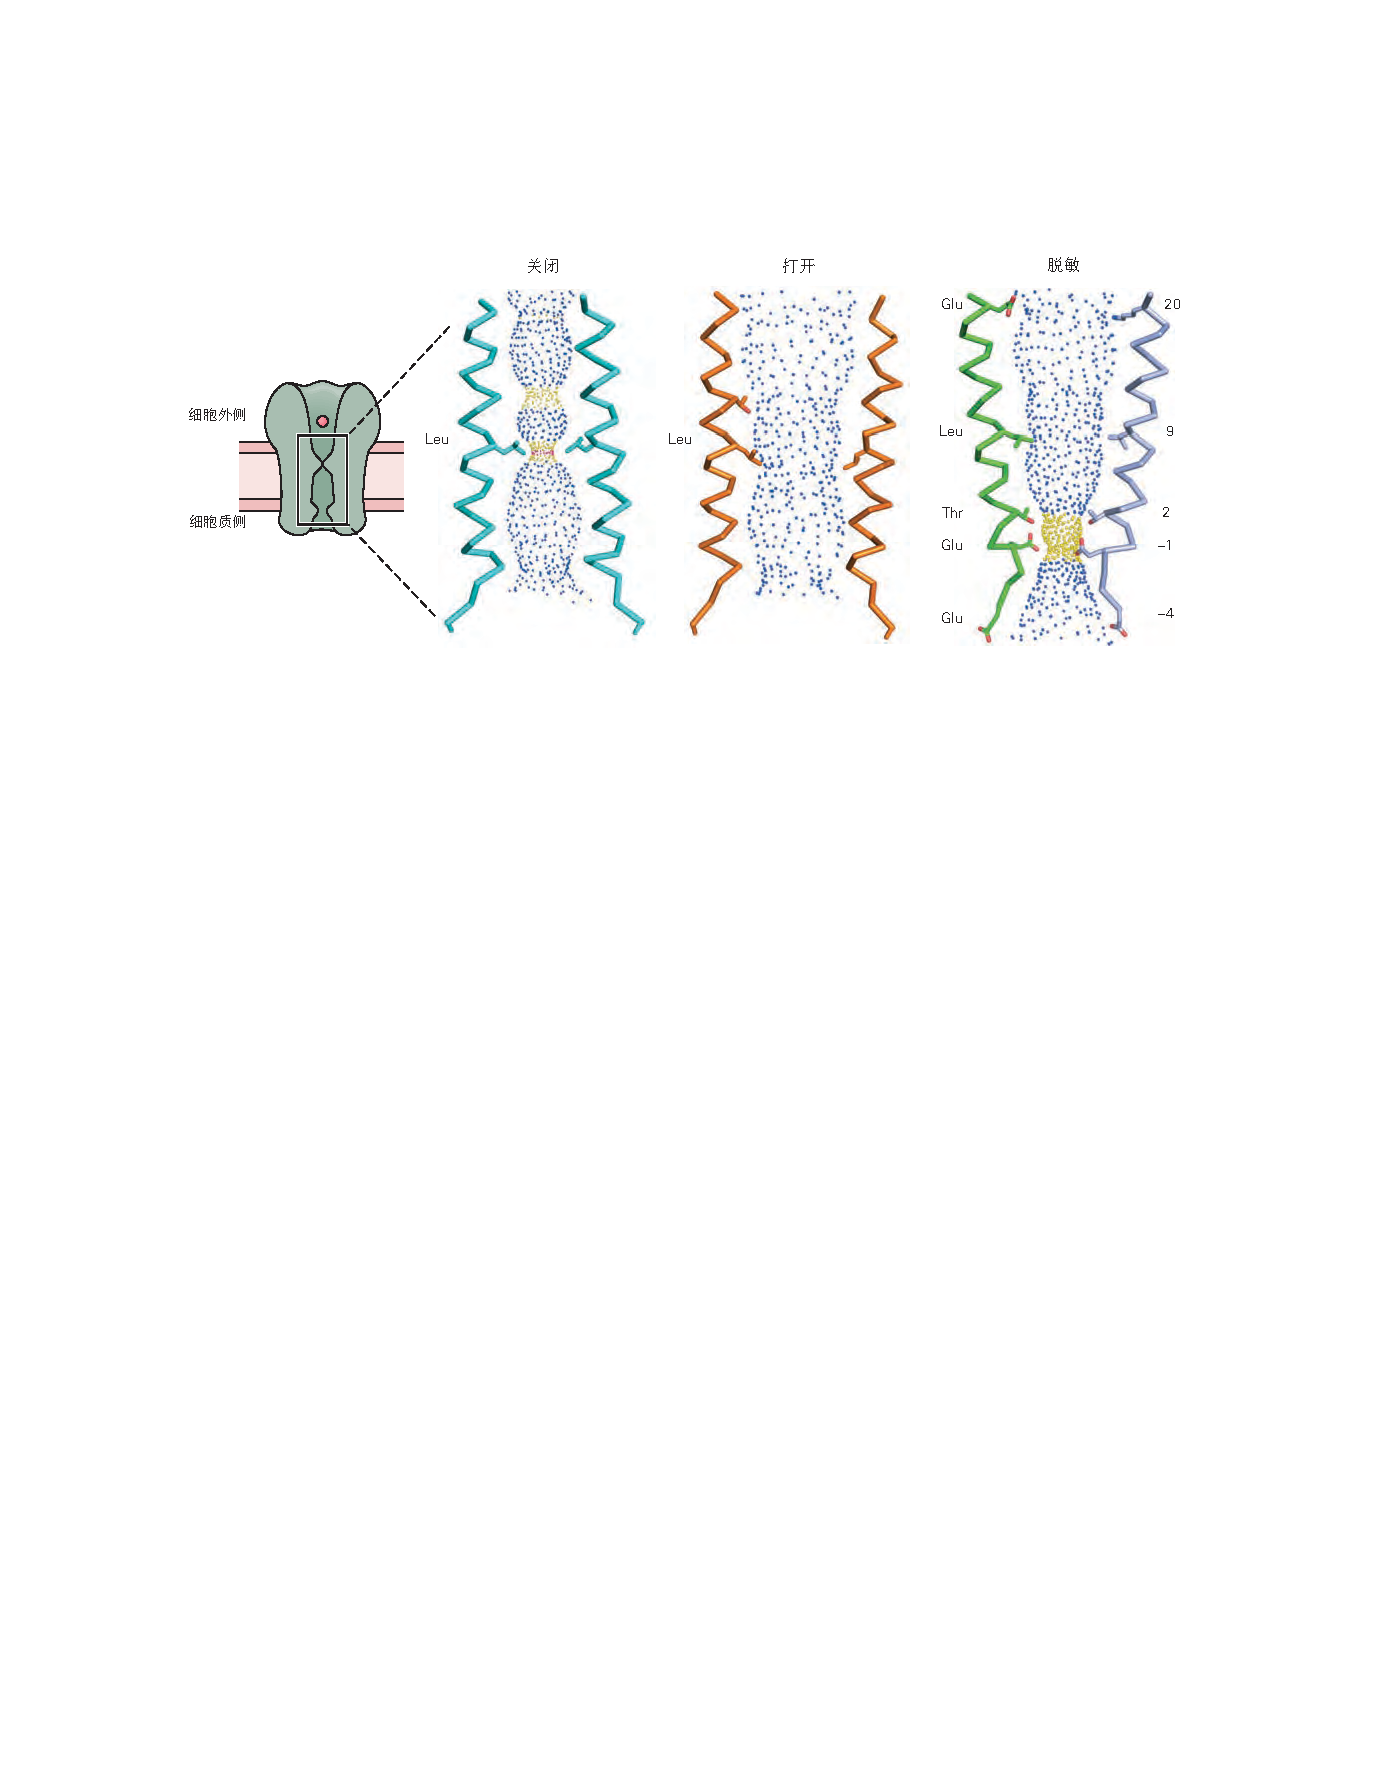
\includegraphics[width=1.0\linewidth]{chap12/fig_12_12}
	\caption{神经元烟碱\textit{乙酰胆碱}受体通道的高分辨率三维结构模型。
		显示了五聚体家族配体门控通道的高分辨率模型,包括受体通道的关闭、打开和脱敏状态。
		显示了五个 M2 $\alpha$-螺旋中的两个。
		脱敏结构来自人类神经元\textit{乙酰胆碱}受体。
		关闭和打开状态基于神经元甘氨酸受体的结构,这些受体在氨基酸序列上与\textit{乙酰胆碱}受体亚基密切相关。
		脱敏\textit{乙酰胆碱}受体的关键氨基酸侧链在右侧显示,位置编号在左侧,氨基酸缩写在左侧。
		按照惯例,位置 0 位于磷脂双分子层的细胞内表面附近;
		其他位置根据一级氨基酸序列中的相对位置进行标记。
		M2 区段中间(位置 9)的保守亮氨酸形成一个门,在关闭状态下收缩孔。
		配体结合导致亚基向外倾斜和扭曲,打开亮氨酸门。
		脱敏过程中的进一步构象变化导致亚基在底部附近向内倾斜,收缩通道细胞内侧附近的孔,从而产生非导电状态。
		位置 20、–1 和 –4 带负电荷的谷氨酸对应于图~\ref{fig:12_11}C 中的外部(1)、中间(2)和内部(3) 电荷环。
		位置–1 位带负电荷的谷氨酸和 2 位带负电的苏氨酸形成通道的选择性过滤器\cite{morales2016x}。}
	\label{fig:12_12}
\end{figure}



\subsection{四大因素决定终板电流}

单个\textit{乙酰胆碱}受体通道携带的矩形电流阶跃如何在终板上产生大的突触电流以响应运动神经刺激?
刺激运动神经会释放大量乙酰胆碱进入突触间隙。
\textit{乙酰胆碱}迅速扩散穿过裂隙并与\textit{乙酰胆碱}受体结合,导致超过 20 万个受体通道几乎同时打开。
( 这个数字是通过比较总终板电流(大约 −500 nA )与通过单个通道的电流(大约 −2.7 pA )获得的)。


这么多通道的快速打开导致终板膜的总电导 $ g_{\text{EPSP}} $ 大幅增加,并产生终板电流的快速上升阶段。
由于间隙中的\textit{乙酰胆碱}迅速减少至零(<1 毫秒),由于酶促水解和扩散,通道开始随机关闭。
尽管每次闭合仅使终板电流呈小的阶梯式下降,但随机闭合大量小的单一电流会导致总终板电流看起来平滑衰减(图~\ref{fig:12_8})。


\begin{figure}[htbp]
	\centering
	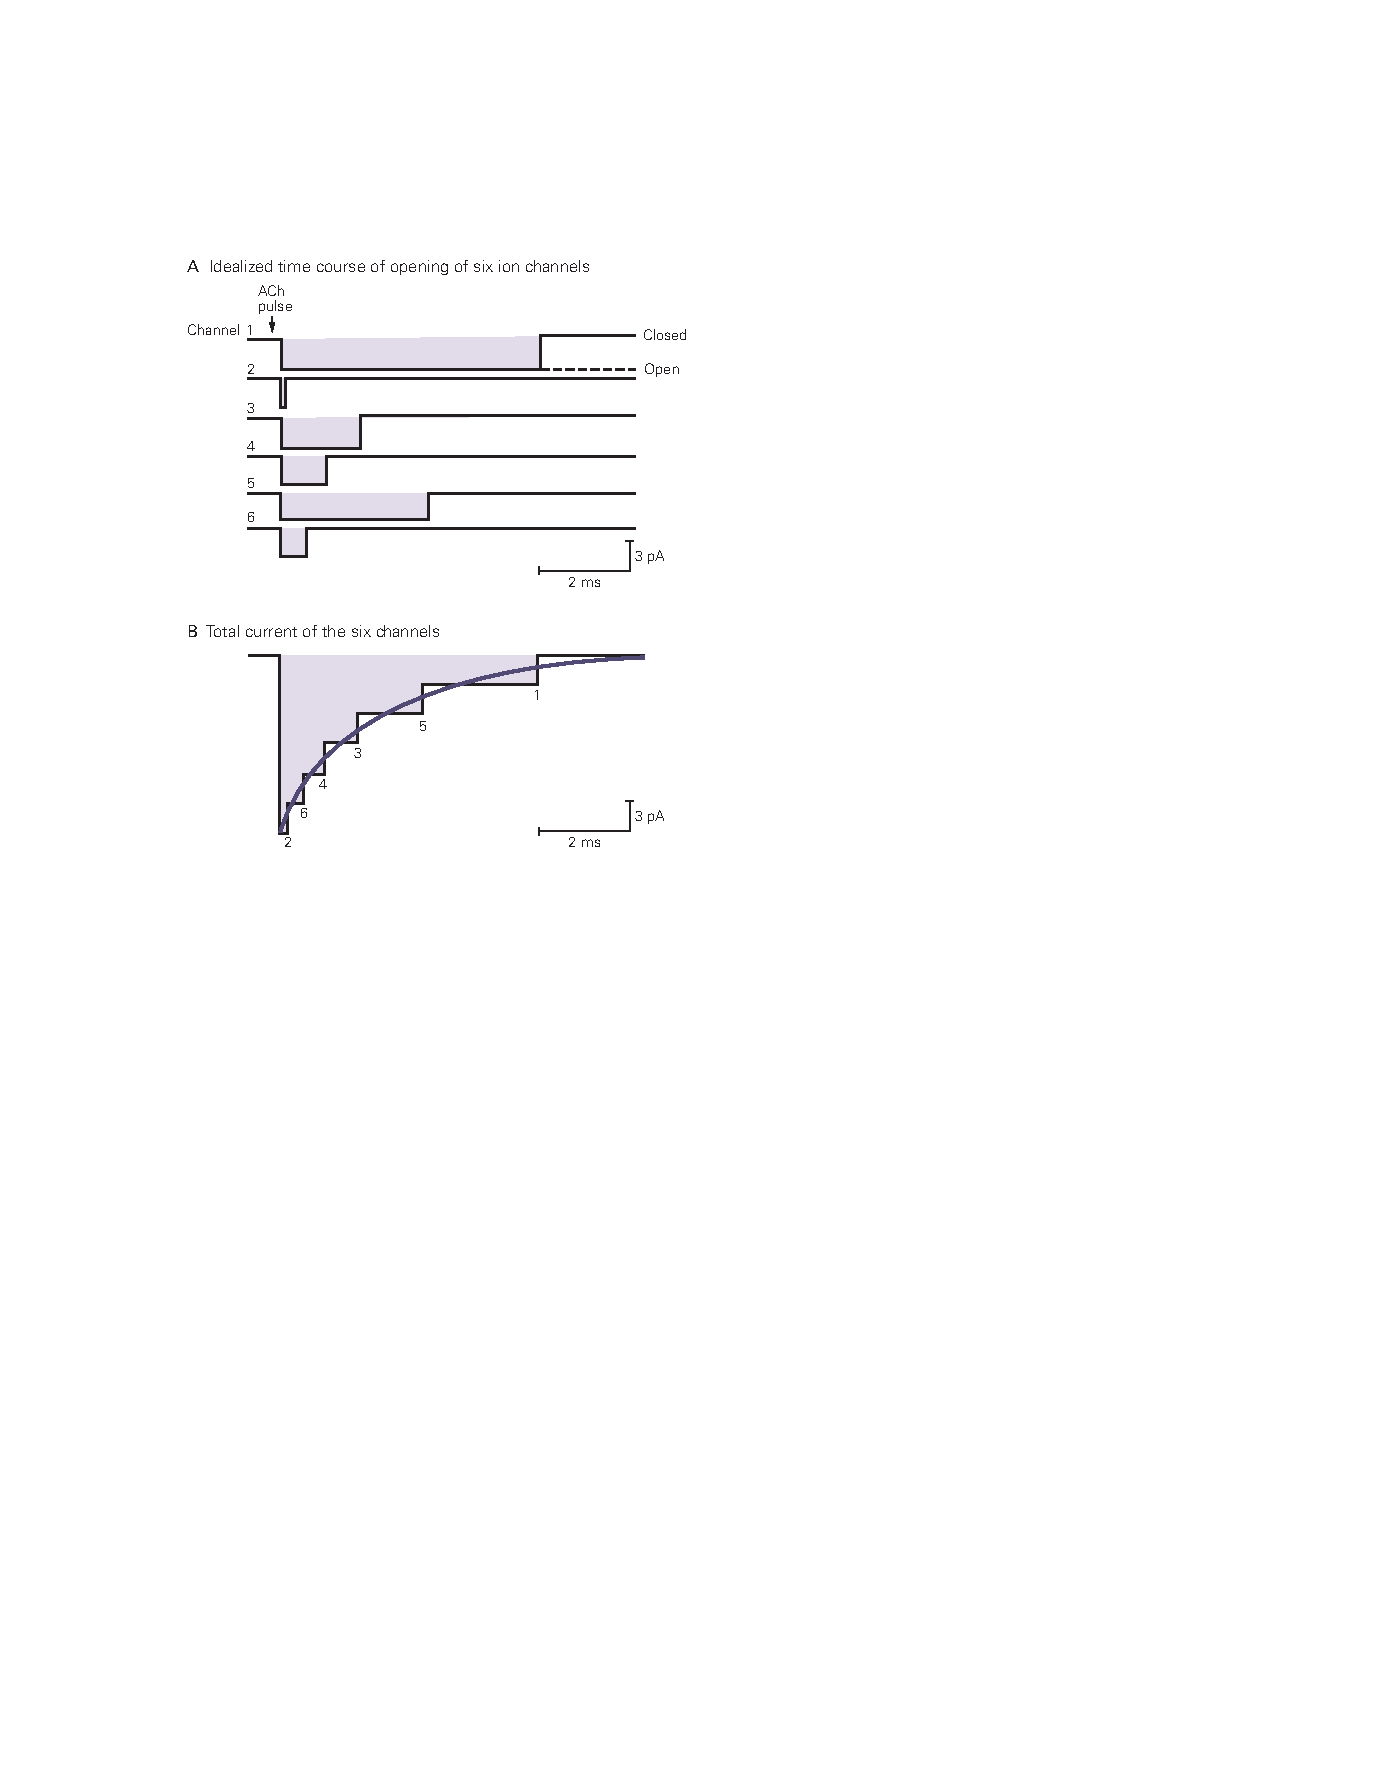
\includegraphics[width=0.65\linewidth]{chap12/fig_12_8}
	\caption{终板总电流的时间进程反映了许多单独的乙酰胆碱受体通道贡献的总和\cite{colquhoun1981fast}。
		\textbf{A.} 个体\textit{乙酰胆碱}受体通道响应\textit{乙酰胆碱}的短暂脉冲而打开。
		在这个理想化的例子中,膜包含六个\textit{乙酰胆碱}受体通道,所有通道都快速且几乎同时打开。
		这些通道在不同时间保持开放,并且独立关闭。
		\textbf{B.} 阶梯迹线为A部分6条单通道电流记录之和,代表各通道依次关闭时的电流( 数字表示关闭的通道)。
		在电流的最后时期,只有一号通道是开放的。
		在整个肌纤维的电流记录中,有数千个通道,无法检测到单个通道关闭,因为显示总终板电流(数百纳安)所需的比例非常大,以至于无法解析出单个通道的贡献。
		因此,总终板电流看起来平稳衰减。}
	\label{fig:12_8}
\end{figure}



\section{乙酰胆碱受体通道具有与产生肌肉动作电位的电压门控通道不同的特性}

产生终板电位的\textit{乙酰胆碱}受体与产生肌肉动作电位的电压门控通道有两个重要区别。
首先,动作电位是由两种不同类别的电压门控通道的顺序激活产生的,一种对 \ce{Na+} 具有选择性,另一种对 \ce{K+} 具有选择性。
相比之下,单一类型的离子通道,即\textit{乙酰胆碱}受体通道,通过允许 \ce{Na+} 和 \ce{K+} 以几乎相等的渗透性通过而产生终板电位。


第二,通过电压门控通道的 \ce{Na+} 流量是可再生的:通过增加细胞的去极化,\ce{Na+} 流入打开更多的电压门控 \ce{Na+} 通道。
这种再生特性决定了动作电位的全有或全无特性。
相比之下,在突触电位期间打开的\textit{乙酰胆碱}受体通道的数量取决于可用的\textit{乙酰胆碱}数量。
\ce{Na+} 通过\textit{乙酰胆碱}门控通道流入产生的去极化不会导致更多\textit{乙酰胆碱}受体通道的打开,也不会产生动作电位。
要触发动作电位,突触电位必须募集相邻的电压门控 \ce{Na+} 通道(图~\ref{fig:12_9})。


\begin{figure}[htbp]
	\centering
	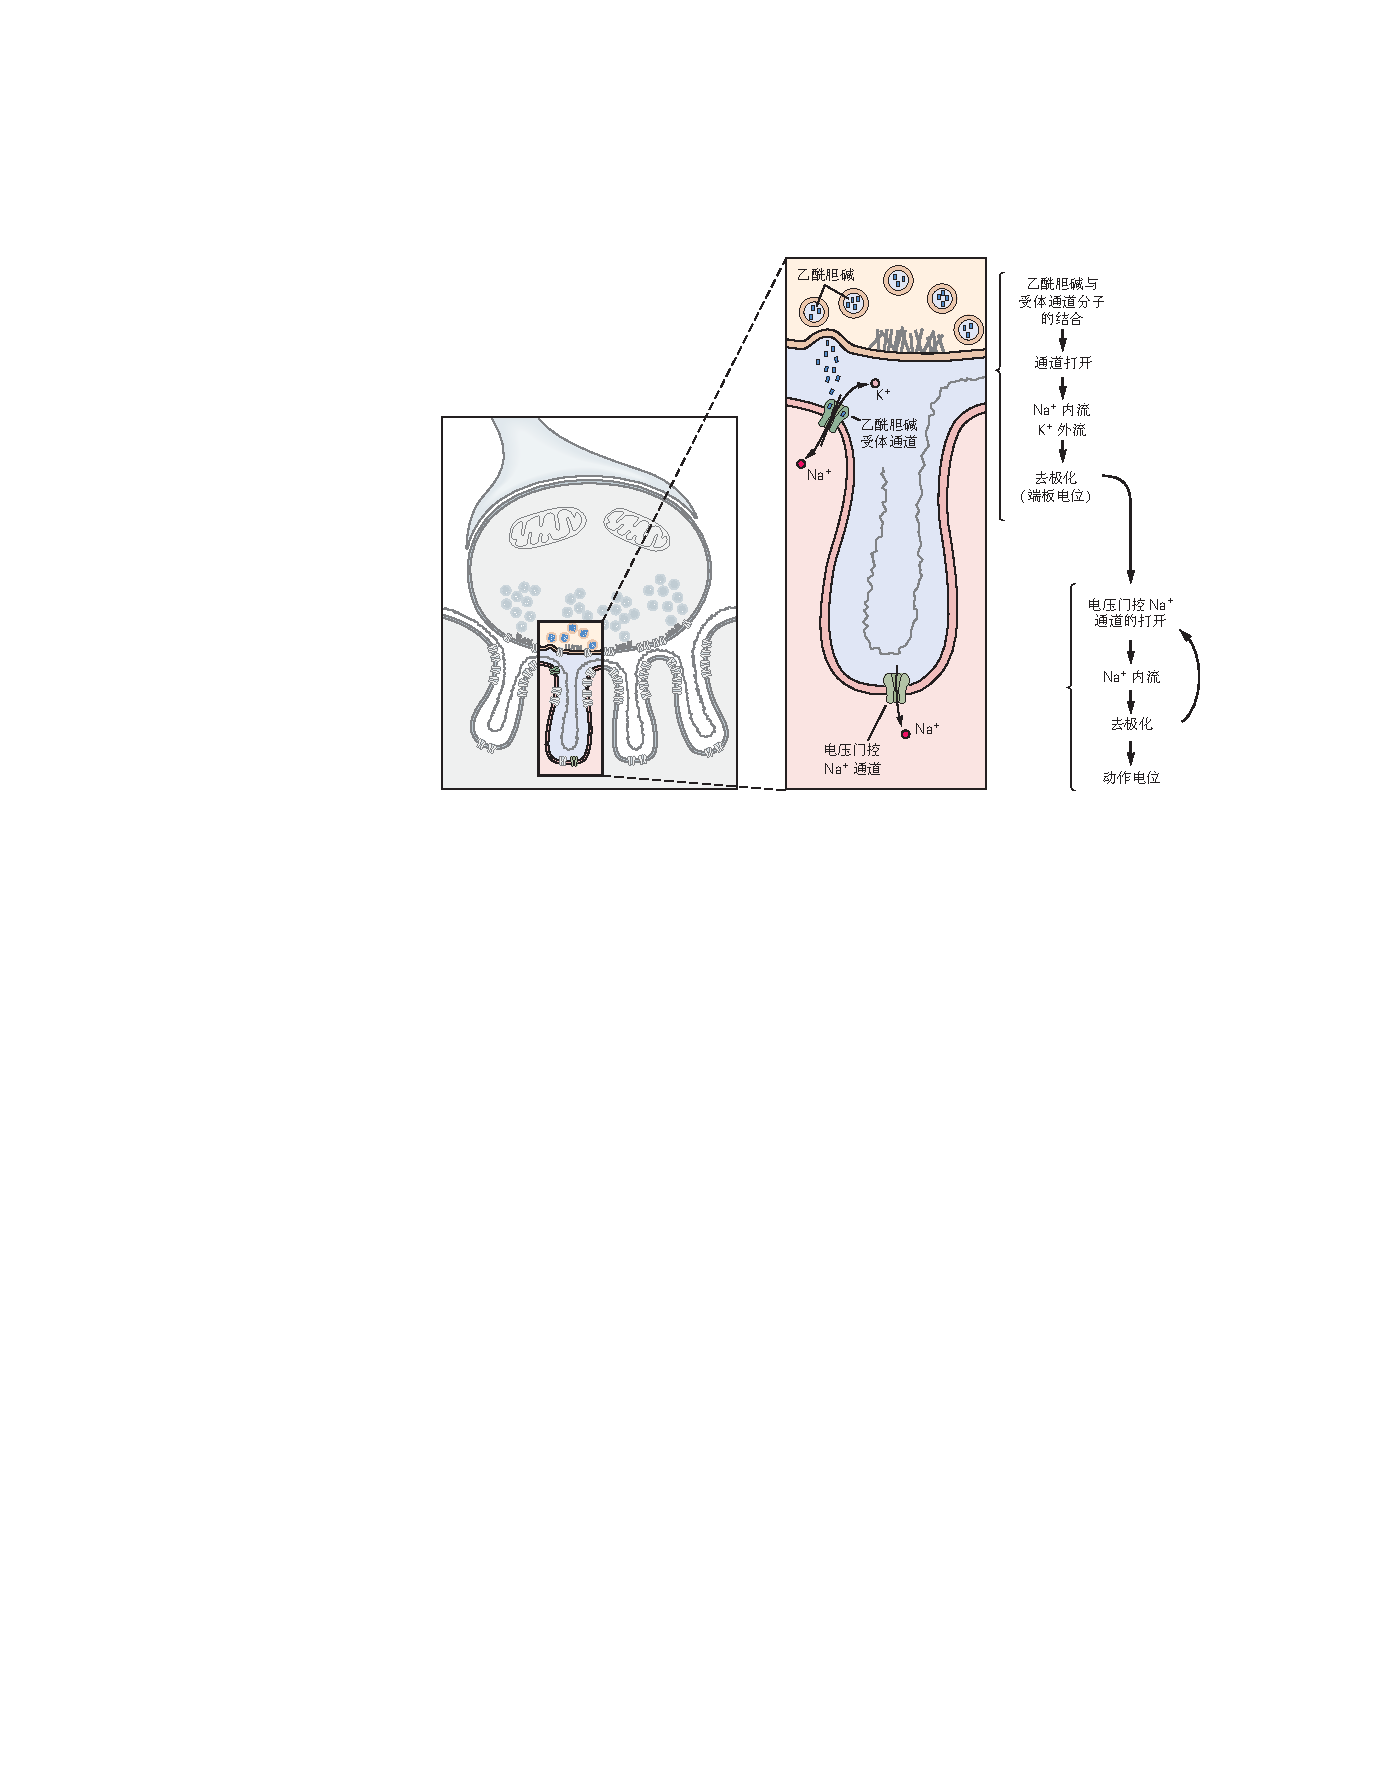
\includegraphics[width=0.9\linewidth]{chap12/fig_12_9}
	\caption{乙酰胆碱受体通道开放导致的终板电位打开电压门控钠通道。
		终板电位通常足够大以打开足够数量的电压门控 \ce{Na+} 通道以超过动作电位的阈值\cite{alberts2017molecular}。}
	\label{fig:12_9}
\end{figure}


正如从这两种生理特性的差异所预期的那样,\textit{乙酰胆碱}受体通道和电压门控通道是由不同的大分子形成的,这些大分子对药物和毒素表现出不同的敏感性。
阻断电压门控 \ce{Na+} 通道的河豚毒素不会阻断 \ce{Na+} 通过烟碱\textit{乙酰胆碱}受体通道流入。
同样,$\alpha$-银环蛇毒素与烟碱受体紧密结合并阻断\textit{乙酰胆碱}的作用,但不干扰电压门控 \ce{Na+} 或 \ce{K+} 通道。



\subsection{递质结合在乙酰胆碱受体通道中产生一系列状态变化}

每个\textit{乙酰胆碱}受体都有两个\textit{乙酰胆碱}结合位点;
两者都必须被发射器占用,通道才能有效打开。
然而,在\textit{乙酰胆碱}的长期应用过程中,通道进入不再传导的脱敏状态。
在正常情况下,肌肉烟碱受体脱敏的时间过程太慢,无法影响\textit{兴奋性突触后电位}的时间过程,其中\textit{乙酰胆碱}仅在非常短的时间内存在于突触间隙中。
然而,脱敏在确定某些神经元突触的突触后反应的时间过程中可以发挥更重要的作用,其中递质可能在突触间隙中持续更长时间或突触后受体经历更快速的脱敏。


例如,\textit{乙酰胆碱}在大脑胆碱能突触的突触间隙中的持续存在可能导致神经元烟碱受体的某些亚型显著脱敏。
重度吸烟者可以积聚足够水平的尼古丁,使大脑中的受体脱敏。
脱敏作用还在药物琥珀酰胆碱的作用中发挥作用,琥珀酰胆碱是\textit{乙酰胆碱}的二聚体,对乙酰胆碱酯酶具有抗性,在全身麻醉期间用于产生肌肉松弛。
琥珀胆碱通过其产生受体脱敏和延长去极化的能力来实现这一点,这通过使电压门控 \ce{Na+} 通道失活来阻断肌肉动作电位。


\textit{卡茨}及其同事首先提出的最小反应模型捕获了\textit{乙酰胆碱}受体通道功能的许多(但不是全部)关键步骤,其中一个闭合的受体通道(R)依次结合两个\textit{乙酰胆碱}分子(A)在经历快速构象变化到开放状态(R*)之前。
随后是非传导脱敏状态(D)的较慢构象变化。
该模型还结合了以下发现,即即使没有\textit{乙酰胆碱},个体受体也有可能进入脱敏状态的可能性很小。
这些结合和门控反应可通过以下方案总结:


现在已经获得\textit{乙酰胆碱}受体所有三种状态的 X 射线晶体结构模型(稍后描述)。



\subsection{分子和生物物理学研究揭示了乙酰胆碱受体的低分辨率结构}

神经肌肉突触处的烟碱\textit{乙酰胆碱}受体是单个大分子的一部分,该大分子包括离子流经的膜孔。
分子中的结合位点位于何处? 通道的孔隙是如何形成的?
\textit{乙酰胆碱}结合如何与通道门控耦合?


从\textit{乙酰胆碱}受体蛋白及其基因的分子和生物物理学研究中获得了对这些问题的见解,首先是从电射线\textit{石纹电鳐}中纯化大分子(图~\ref{fig:12_2})。
使用不同的生化方法,\textit{亚瑟$\cdot$卡林}和\textit{让$\cdot$皮埃尔$\cdot$尚热}从电斑中纯化了受体,电斑是专门的肌肉样细胞,其堆叠状包装使它们各自的\textit{兴奋性突触后电位}串联求和以产生大电压(>100 伏特),用于电击猎物。
他们的研究表明,成熟的烟碱\textit{乙酰胆碱}受体是一种膜糖蛋白,由五个分子量相似的亚基组成:两个 $\alpha$-亚基和一个 $\beta$-、一个 $\gamma$- 和一个 $\delta$-亚基(图~\ref{fig:12_10})。


\begin{figure}[htbp]
	\centering
	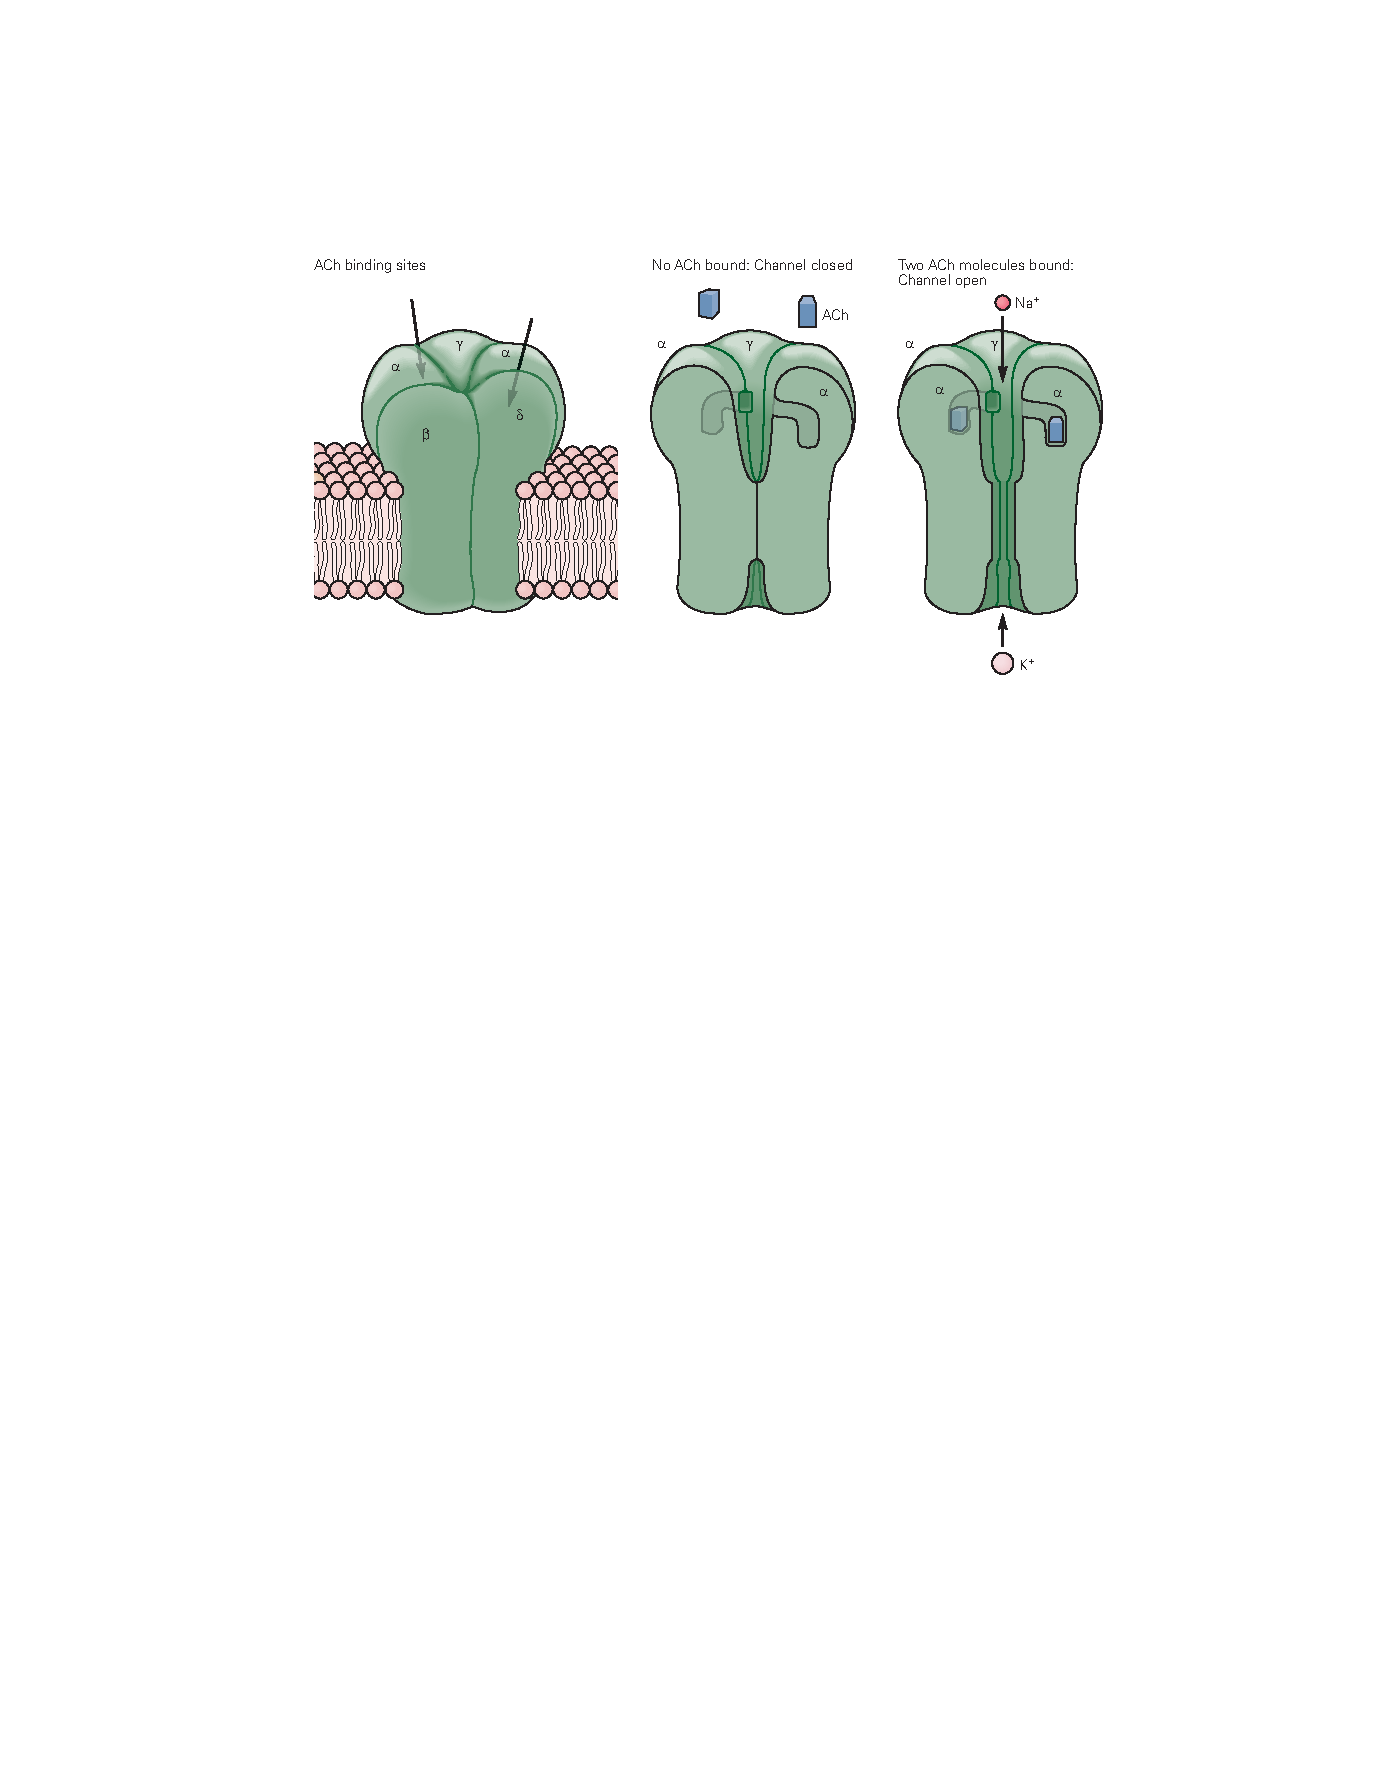
\includegraphics[width=0.95\linewidth]{chap12/fig_12_10}
	\caption{烟碱型\textit{乙酰胆碱}受体通道是一种五聚体大分子。
		受体和通道是单个大分子的组成部分,该大分子由五个亚基组成:
		两个相同的 $\alpha$-亚基和 $\beta$-、$\gamma$- 和 $\delta$-亚基各一个。
		亚基形成穿过细胞膜的孔。
		当两个\textit{乙酰胆碱}分子与细胞外结合位点结合时(在两个 $\alpha$-亚基及其相邻的 $\gamma$- 和 $\delta$-亚基的界面处形成),受体通道分子的构象发生变化(见图~\ref{fig:12_12})。
		这种变化打开了 \ce{K+} 和 \ce{Na+} 沿其电化学梯度向下流动的孔隙。}
	\label{fig:12_10}
\end{figure}


\textit{卡林}和他的同事在每个 $\alpha$-亚基与其相邻的 $\gamma$- 或 $\delta$-亚基之间的裂隙中的每个受体蛋白上确定了\textit{乙酰胆碱}的两个细胞外结合位点。
一个\textit{乙酰胆碱}分子必须结合两个位点中的每一个,通道才能有效打开(图~\ref{fig:12_10})。
由于 $\alpha$-银环蛇毒素与\textit{乙酰胆碱}一样与 $\alpha$-亚基上的相同结合位点紧密结合,因此该毒素充当不可逆的递质拮抗剂。


对\textit{乙酰胆碱}受体通道结构的进一步了解来自对受体四个不同亚基的一级氨基酸序列的分析和生物物理学研究。
\textit{沼正作}及其同事的分子克隆表明,这四个亚基由不同但相关的基因编码。
亚基的序列比较显示出高度的相似性(一半的氨基酸残基相同或被保守取代),这表明所有亚基都具有相似的结构。 
此外,所有四个亚基基因都是同源的;
也就是说,它们源自共同的祖先基因。
神经元中的烟碱\textit{乙酰胆碱}受体由一组不同但相关的基因编码。
所有这些受体都是五聚体;
然而,它们的亚基组成和化学计量各不相同。
大多数神经元受体由两个 $\alpha$ 亚基和三个 $\beta$ 亚基组成,而一些神经元受体由五个相同的 $\alpha$ 亚基($\alpha$7 亚型)组成,因此可以结合五个\textit{乙酰胆碱}分子。


所有烟碱\textit{乙酰胆碱}受体亚基在\textit{乙酰胆碱}的细胞外结合位点附近都包含一个高度保守的序列,该序列由两个二硫键结合的\textit{半胱氨酸}残基和 13 个中间氨基酸组成。
由此产生的 15 氨基酸环形成了烟碱\textit{乙酰胆碱}受体亚基和神经元中其他递质的相关受体的特征序列。
\textit{半胱氨酸}环受体家族,也称为\textit{五聚体配体门控离子通道},包括神经递质 \textit{$\gamma$-氨基丁酸}、甘氨酸和血清素的受体。


亚基的极性和非极性氨基酸的分布提供了关于亚基如何穿过膜双层的第一条线索。
每个亚基包含四个大约由 20 个氨基酸组成的疏水区域,称为 M1 到 M4,每个区域形成一个跨膜的 $\alpha$ 螺旋(图~\ref{fig:12_11}A)。
亚基的氨基酸序列表明亚基的排列使得它们在膜上形成一个中心孔(图~\ref{fig:12_11} B)。


\begin{figure}[htbp]
	\centering
	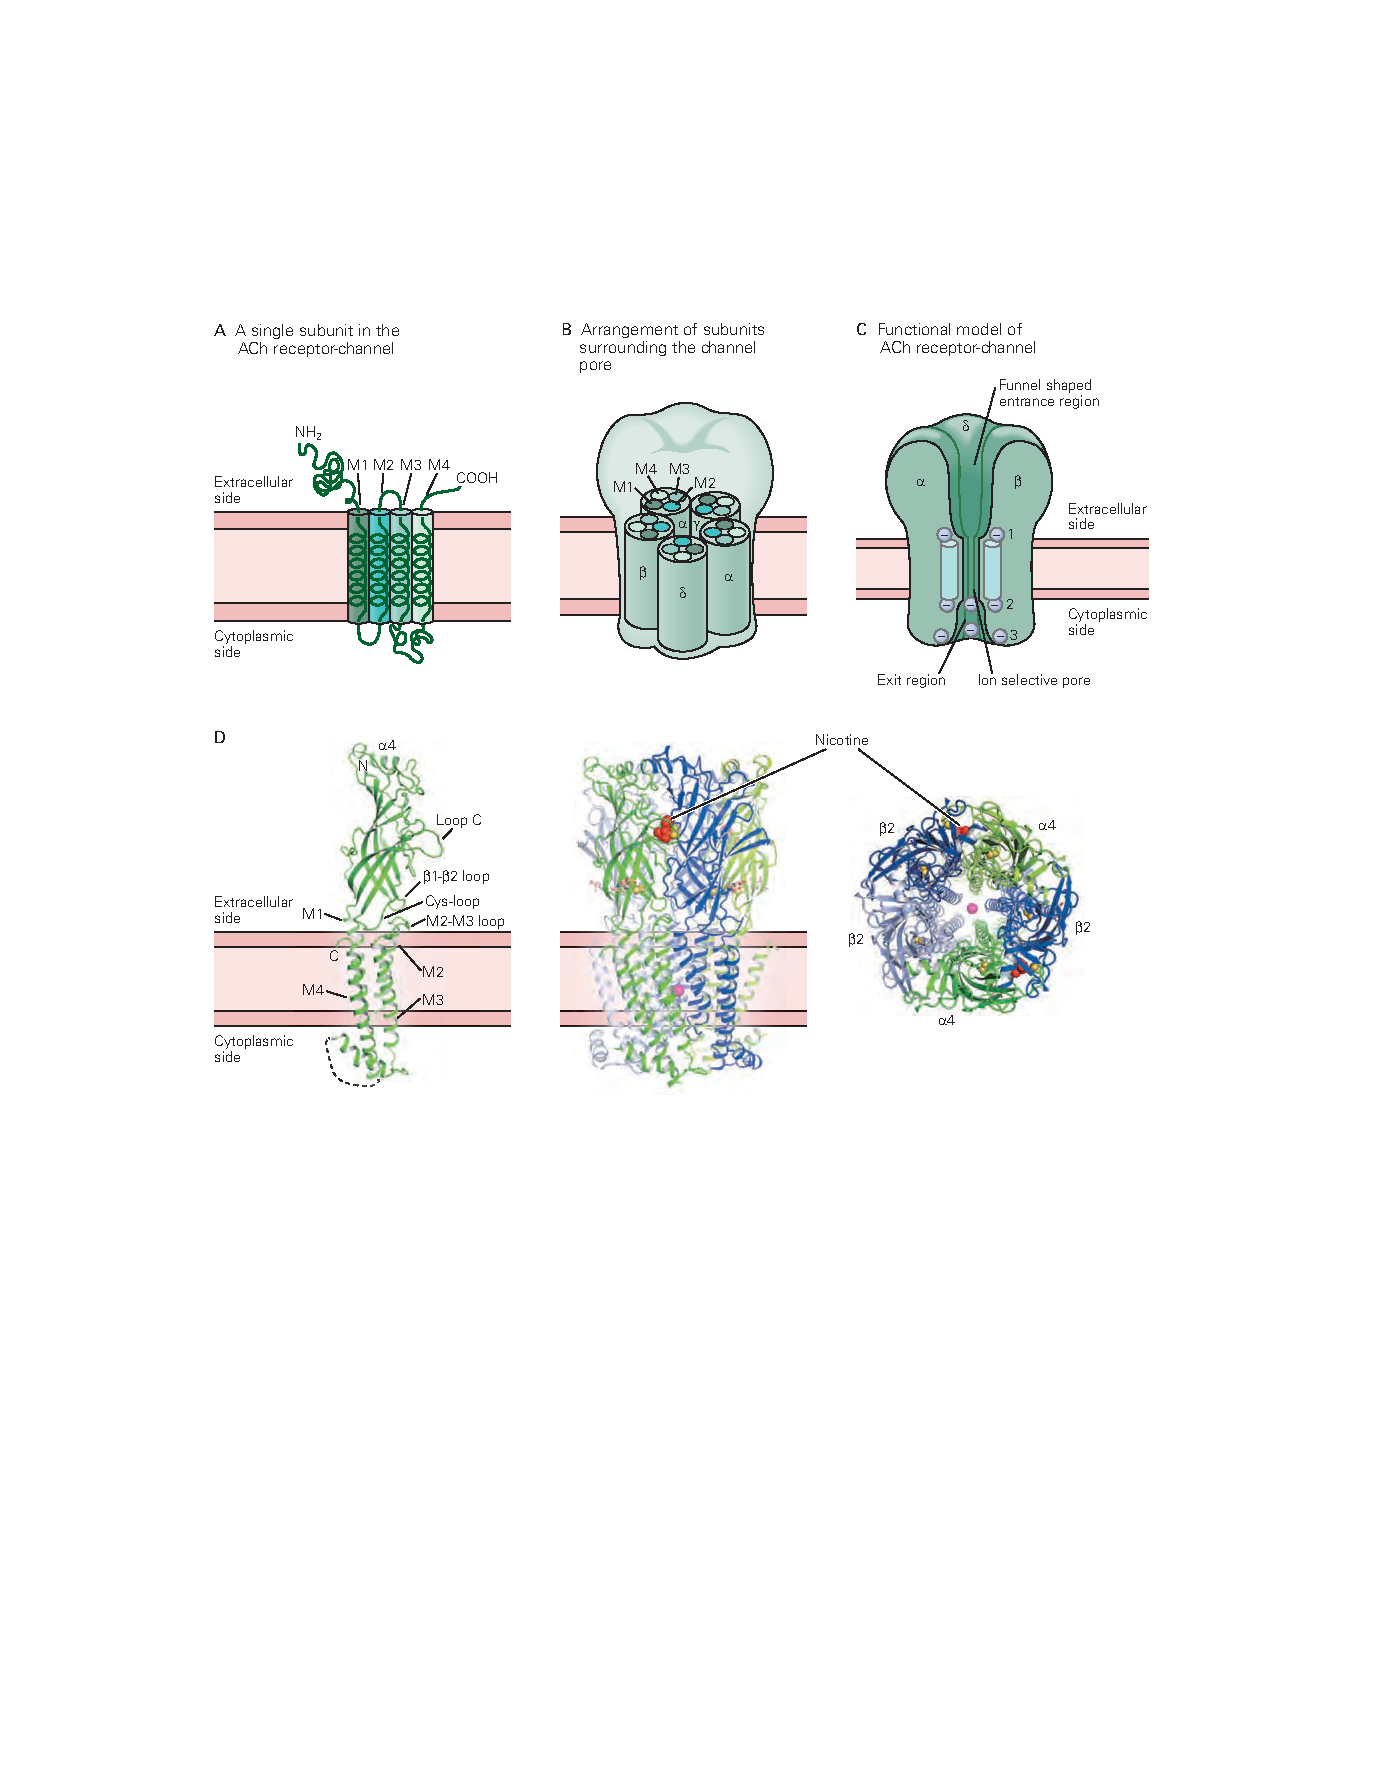
\includegraphics[width=1.0\linewidth]{chap12/fig_12_11}
	\caption{\textit{乙酰胆碱}受体亚基是同源的跨膜蛋白。
		\textbf{A.} 每个亚基都包含一个大的细胞外 N 末端、四个跨膜 $\alpha$ 螺旋(M1–M4)和一个短的细胞外 C 末端。
		N 端包含\textit{乙酰胆碱}结合位点,膜螺旋形成孔。
		\textbf{B.} 五个亚基的排列使得它们形成一个中央水通道,每个亚基的 M2 部分形成孔的内层。
		$\gamma$亚基位于两个$\alpha$亚基之间。 (尺寸未按比例绘制。)
		\textbf{C.} 每个亚基上带负电荷的氨基酸在孔周围形成三个带负电荷的环。
		当离子穿过通道时,它会遇到这些电荷环。
		细胞膜内外表面的环(1, 3)可用作预滤器,帮助排斥阴离子并形成二价阳离子阻断位点。
		膜双层(2)细胞质侧附近的中心环可能更重要地有助于建立选择性过滤器的特定阳离子选择性,这是孔的最窄区域。
		\textbf{D.} 人类神经元烟碱\textit{乙酰胆碱}受体通道的高分辨率 X 射线晶体结构模型。
		右图:开放通道的俯视图,由围绕中心孔排列的两个 a4 亚基和三个 b2 亚基组成。
		这些亚基是肌肉受体的$\alpha$和$\beta$亚基的密切相关变体。
		两个尼古丁分子(显示为红色球体的原子)与受体结合。
		渗透阳离子显示为粉红色球体。
		中心:受体的侧视图,显示膜的磷脂双层和结合尼古丁的位置。
		左图:膜平面中单个$\alpha$亚基的侧视图。
		该亚基的氨基末端由一个大的细胞外结构域组成。
		环 C 有助于形成配体结合位点。
		胞外域和 M1-M4 跨膜 $\alpha$ 螺旋之间界面处的 $\beta$1-$\beta$2 和半胱氨酸环将构象变化从配体结合位点传递到孔以打开通道\cite{morales2016x}。}
	\label{fig:12_11}
\end{figure}


通道孔壁由 M2 跨膜段和连接 M2 和 M3 的环路形成。
位于 M2 区段内外边界两侧的三个负电荷环在通道对阳离子的选择性中起着重要作用。
某些局部麻醉药通过与膜中途 M2 螺旋中心区域的一个极性丝氨酸残基环和两个疏水性残基环相互作用来阻断通道。


整个受体通道复合体的三维模型最初由\textit{卡林}基于低分辨率中子散射和\textit{奈杰尔$\cdot$昂温}基于电子衍射图像提出。
该复合体分为三个区域:包含\textit{乙酰胆碱}结合位点的大细胞外部分、对阳离子具有选择性的窄跨膜孔和内膜表面的大出口区域(图~\ref{fig:12_11} C)。
细胞外区域非常大,长度约为 6 纳米。
此外,孔的细胞外端有一个直径约为 2.5 纳米的宽口。
在膜的双层内,孔逐渐变窄。


自身免疫性疾病重症肌无力是由与\textit{乙酰胆碱}受体胞外结构域结合的抗体的产生引起的,导致神经肌肉接头处烟碱型\textit{乙酰胆碱}受体的数量或功能下降。
如果变化足够严重,这可能会将\textit{兴奋性突触后电位}降低到触发动作电位的阈值以下,从而导致虚弱无力。
几种先天性肌无力形式是由烟碱\textit{乙酰胆碱}受体亚基突变引起的,这些亚基也可以改变受体数量或通道功能。
例如,M2 区段氨基酸残基的突变会导致通道开放时间延长,称为慢通道综合症,这会导致过度的突触后兴奋,从而导致终板退化(第~\ref{chap:chap57} 章)。



\subsection{X 射线晶体研究揭示了乙酰胆碱受体通道的高分辨率结构}

对\textit{乙酰胆碱}结合位点细节的更深入了解最初来自软体动物\textit{乙酰胆碱}结合蛋白的高分辨率 X 射线晶体学研究,该蛋白与烟碱\textit{乙酰胆碱}受体亚基的细胞外氨基末端同源。
值得注意的是,与典型的\textit{乙酰胆碱}受体不同,软体动物\textit{乙酰胆碱}结合蛋白是由神经胶质细胞分泌到细胞外空间的可溶性蛋白。
在蜗牛的胆碱能突触中,它可以减小\textit{兴奋性突触后电位}的大小,这可能是通过缓冲突触间隙中\textit{乙酰胆碱}的游离浓度。


对完整受体通道结构的进一步了解来自细菌和多细胞动物的相关五聚体配体门控通道的 X 射线晶体结构,最终以复杂的人神经元烟碱\textit{乙酰胆碱}受体的最近 X 射线晶体结构达到顶峰 与尼古丁。
结合相关蛋白质的结构知识,我们现在对\textit{乙酰胆碱}受体通道和相关配体门控通道的配体结合、通道门控和离子渗透的结构和机制有了非常详细的了解。


在神经元\textit{乙酰胆碱}受体中,两个 $\alpha$-亚基与三个 $\beta$-亚基结合形成五聚体(图~\ref{fig:12_11}D)。
受体的大细胞外结构域包含两个\textit{乙酰胆碱}结合位点,并形成一个五聚体环,围绕着一个大的中央前庭,这可能将离子汇集到受体的狭窄跨膜结构域。
每个 $\alpha$-亚基在位于与相邻 $\beta$-亚基界面的位点结合一个尼古丁分子。
来自\textit{奈杰尔$\cdot$昂温}的相关\textit{半胱氨酸}环受体的高分辨率结构和神经元烟碱受体脱敏状态的高分辨率结构的电子衍射数据表明,每个亚基的四个跨膜区段确实是穿过 3 纳米的 $\alpha$ 螺旋 脂质双层的长度(图~\ref{fig:12_12})。
在脱敏状态下,来自五个亚基的 M2 区段在膜的细胞内侧附近形成狭窄的收缩,阻止离子渗透。


我们对处于打开和关闭状态的烟碱\textit{乙酰胆碱}受体通道的跨膜区域的描述仍然不完整。
然而,与相关\textit{五聚体配体门控离子通道}的结构相比,受体的连贯图景开始出现。
在闭合状态下,孔衬里的 M2 段彼此大致平行,形成一个狭窄的中央孔。
M2 区段中间附近的一圈高度保守的疏水性亮氨酸残基将孔进一步收缩至直径 0.3 至 0.4 纳米(图~\ref{fig:12_12})。
这种疏水收缩被认为提供了一个高能屏障,限制直径大于孔中收缩的水合阳离子的通过。
目前,从电生理测量(0.6 纳米)推断的孔径差异与从晶体结构得出的较窄值仍未解决。


在开放状态下,M2 片段被认为向外倾斜并旋转,扩大了 M2 中间亮氨酸残基的收缩,从而实现离子渗透。
开放孔中最窄的收缩位于通道的细胞内口附近,其中来自一个苏氨酸残基环(肌肉\textit{乙酰胆碱}受体中的丝氨酸和苏氨酸残基)和第二个带负电荷的谷氨酸残基环的负电羟基侧链被认为 形成选择性滤波器。
在脱敏状态下,M2 部分进一步倾斜,导致选择性过滤器收缩得更多,从而阻止离子渗透。


基于各种结构和功能研究,现在正在出现配体结合如何导致通道开放的详细图片。
配体的结合被认为可以促进相邻亚基之间裂缝的闭合,从而导致五聚体的细胞外结构域收紧,类似于花瓣的闭合。
这导致扭转运动,导致受体细胞外结构域的底部推动 M1 区段和连接 M2 和 M3 跨膜区段的细胞外环。
该运动对 M2 段施加力,导致其旋转和倾斜,从而打开孔中间的疏水亮氨酸门并允许离子渗透。
尽管未来的研究无疑将完善我们对烟碱受体通道和功能的结构基础的理解,但这些最新进展使我们对神经系统中最基本的过程之一有了前所未有的分子理解:
突触传递,特别是信号传导从神经到肌肉的信息。



\section{亮点}

1. 运动神经元的末端在称为终板的肌膜特殊区域与肌纤维形成突触。
当动作电位到达突触前运动神经元的末端时,它会导致\textit{乙酰胆碱}的释放。 


2. \textit{乙酰胆碱}在几微秒内扩散穿过狭窄的(100 纳米)突触间隙,并与终板膜中的烟碱\textit{乙酰胆碱}受体结合。
结合能量转化为构象变化,打开蛋白质中的阳离子选择性通道,允许 \ce{Na+}、\ce{K+} 和钙离子流过突触后膜。
主要由于 \ce{Na+} 离子的流入,净效应产生称为终板电位的去极化突触电位。 


3. 因为\textit{乙酰胆碱}受体通道集中在终板,这些通道的打开会产生局部去极化。
这种局部去极化足够大(75 毫伏),超过动作电位产生的阈值三到四倍。 


4.重要的是神经肌肉传递的安全系数要高,因为它决定了我们移动、呼吸和逃生的能力。
自身免疫性疾病或基因突变导致的\textit{乙酰胆碱}受体数量或功能下降可能导致神经系统疾病。 


5. 膜片钳记录揭示了电流对单个\textit{乙酰胆碱}受体通道的打开和关闭的阶梯式增加和减少。
神经肌肉接头处典型的兴奋性突触后电流是由大约 20 万个单独通道的打开产生的。 


6. 肌肉烟碱\textit{乙酰胆碱}受体的生化结构已经确定。
该受体是由两个 $\alpha$-亚基和一个 $\beta$-$\gamma$-和 $\delta$-亚基组成的五聚体。
编码亚基的四个基因与编码其他发射器的其他五聚体配体门控通道的基因密切相关,并且关系更远。 


7. 更高分辨率的结构提供了\textit{乙酰胆碱}配体结合口袋和通道孔的详细视图,并进一步深入了解配体结合如何导致与受体通道开放和脱敏门控反应相关的构象变化。


\section{后记:端板电流可由等效回路计算}

通过\textit{乙酰胆碱}受体通道的电流可以用欧姆定律来描述。
然而,为了描述电流如何产生终板电位,还必须考虑周围膜中静息通道的电导。
我们还必须考虑由细胞内外的 \ce{Na+} 和 \ce{K+} 分布决定的膜和离子电池的电容特性。


这些不同组件之间的动态关系可以使用我们在第~\ref{chap:chap9}~章中用于分析仅由电阻器、电容器和电池组成的无源电气设备中的电流的相同规则来解释。
我们可以用具有三个平行电流路径的等效回路来表示终板区域:
(1)一个用于通过发射机门控通道的突触电流,
(2)一个用于通过静息通道(非突触膜)的返回电流 ,和
(3)一个用于脂质双层的电容电流(图~\ref{fig:12_13})。
为简单起见,我们忽略了周围非突触膜中的电压门控通道。


\begin{figure}[htbp]
	\centering
	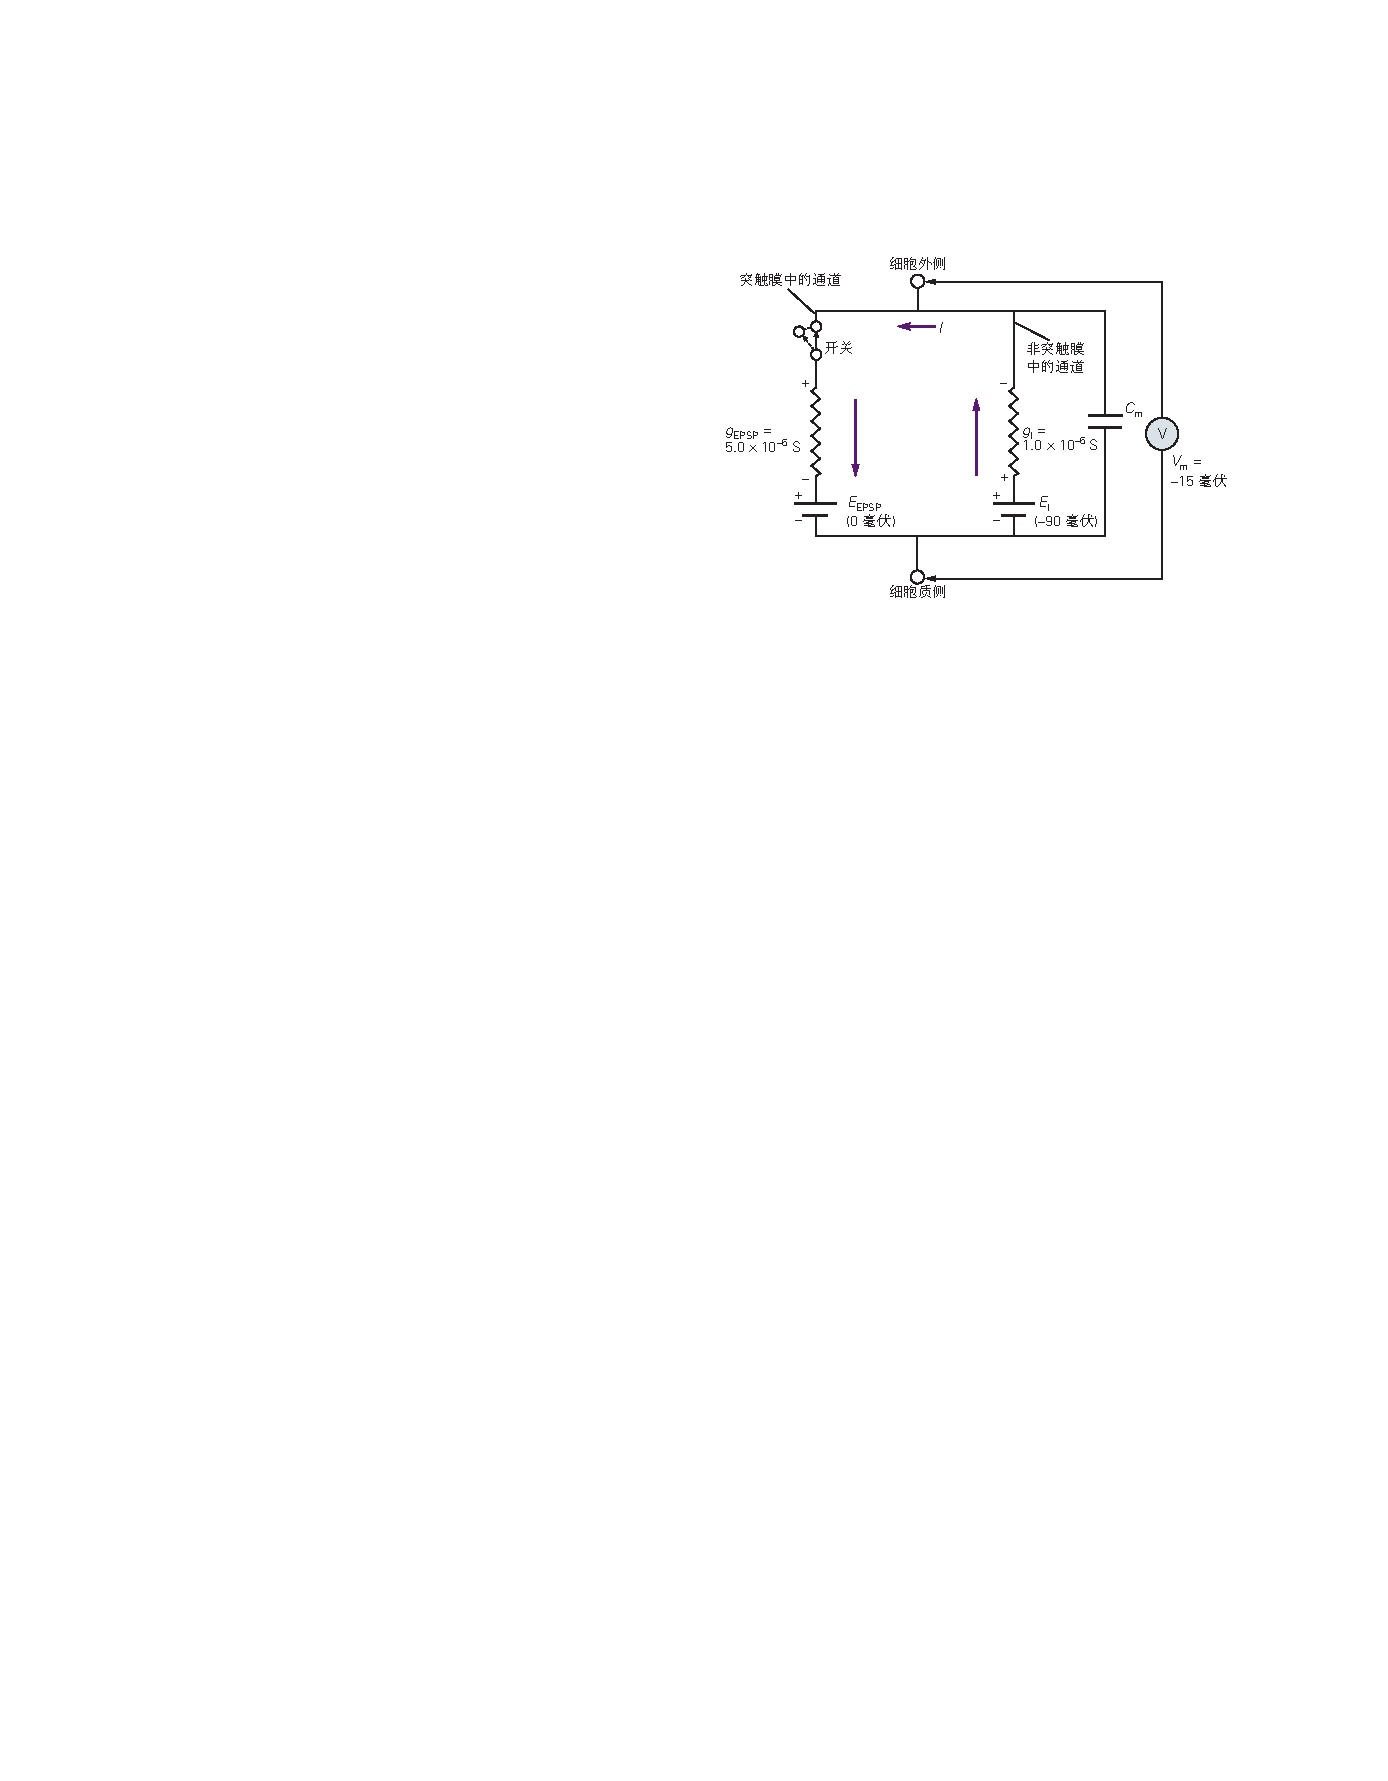
\includegraphics[width=0.6\linewidth]{chap12/fig_12_13}
	\caption{端板的等效回路。
		该回路具有三个并联电流通路。
		一种电导通路承载终板电流,由与\textit{乙酰胆碱}受体通道($ g_{\text{EPSP}} $)的电导串联的细胞($E_{\text{EPSP}}$)组成。
		另一个电导通路携带电流通过非突触膜,由代表静息电位($ E_l $)的电池与静息通道的电导($ g_l $)串联组成。
		与这两个电导通路并联的是膜电容($ C_m $)。
		电压表(V)测量电池内部和外部之间的电位差。
		当不存在\textit{乙酰胆碱}时,\textit{乙酰胆碱}受体通道关闭并且不携带电流。
		这种状态被描述为一个开路回路,其中突触电导没有连接到回路的其余部分。
		\textit{乙酰胆碱}的结合打开突触通道。
		此事件在电气上等效于打开连接门控电导通路($ g_{\text{EPSP}} $)与静息通路($ g_l $)的开关。
		在稳定状态下,通过\textit{乙酰胆碱}受体通道的内向电流与通过静息通道的外向电流平衡。
		根据电导和电池的指示值,膜将从 −90 毫伏(其静息电位)去极化至 −15 毫伏(终板电位的峰值)。}
	\label{fig:12_13}
\end{figure}


因为终板电流由流经同一离子通道的 \ce{Na+} 和 \ce{K+} 携带,我们将 \ce{Na+} 和 \ce{K+} 电流通路组合成一个代表\textit{乙酰胆碱}受体通道的电导($ g_{\text{EPSP}} $)。
该通路的电导率与打开的通道数成正比,而打开的通道数又取决于突触间隙中递质的浓度。
在没有发射器的情况下,没有通道打开并且电导为零。
当突触前动作电位导致\textit{乙酰胆碱}释放时,该通路的电导增加到大约 $ 5 \times 10^{-6} $ S,大约是代表静息(泄漏)通道($ g_l $)的平行分支电导的五倍。


终板电导与细胞($E_{\text{EPSP}}$)串联,其值由突触电流(0 毫伏)的反转电位给出(图~\ref{fig:12_13})。
该值是 \ce{Na+} 和 \ce{K+} 平衡电位的加权代数和(见方框~\ref{box:12_1})。
兴奋性突触后电位($I_{\text{EPSP}}$)期间的电流由下式给出


\begin{equation}\label{excitatory_potential}
	L_{\text{EPSP}} = g_{\text{EPSP}} \times (V_m - E_{\text{EPSP}}).
\end{equation}


使用这个等式和图~\ref{fig:12_13}~的等效回路,我们现在可以根据其组件分析\textit{兴奋性突触后电位}(图~\ref{fig:12_14})。


\begin{figure}[htbp]
	\centering
	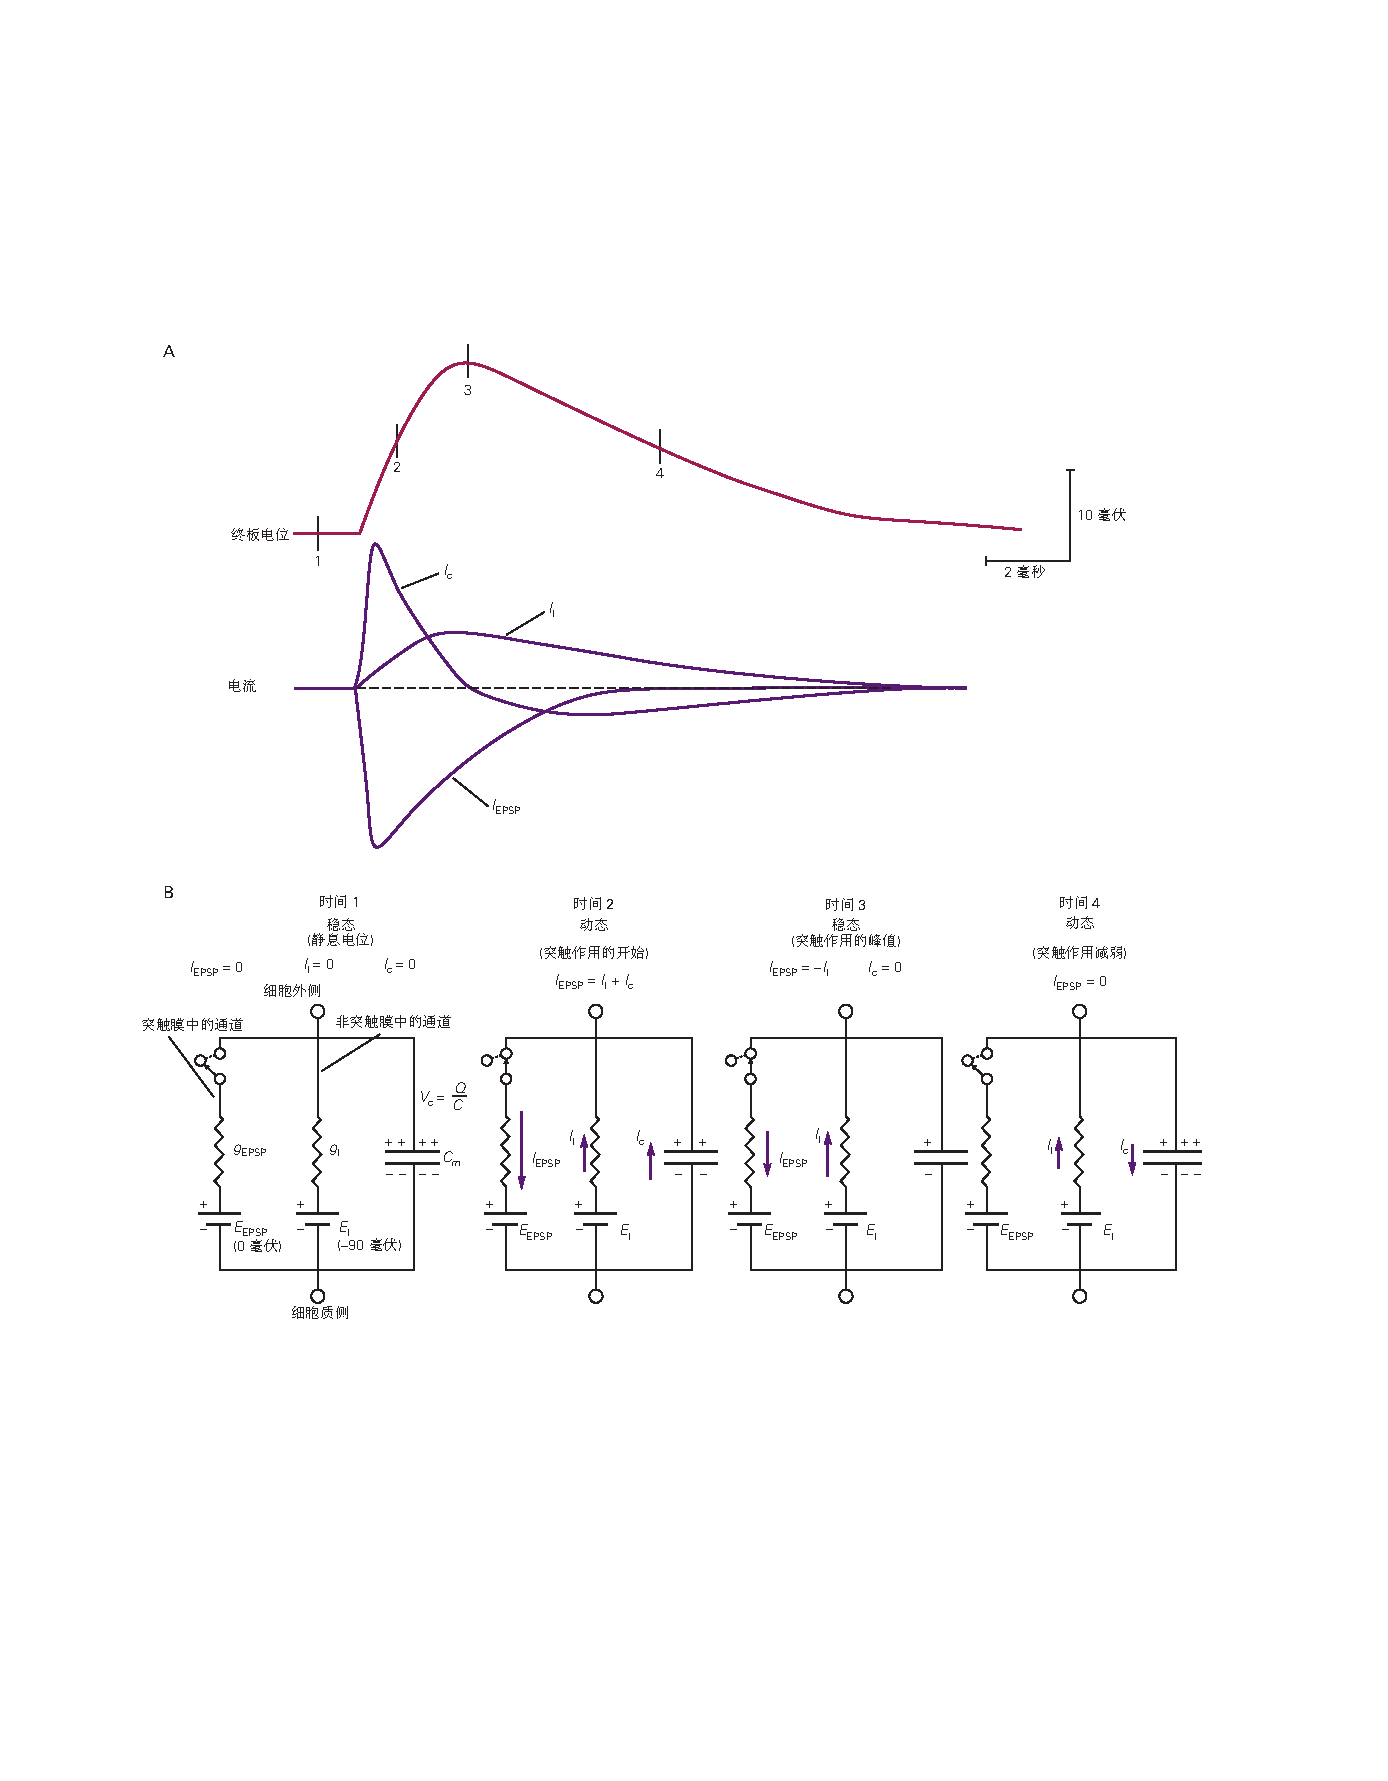
\includegraphics[width=1.0\linewidth]{chap12/fig_12_14}
	\caption{终板电位的时间进程由\textit{乙酰胆碱}门控突触电导和肌肉细胞的被动膜特性决定。
		\textbf{A.} 终板电位和通过\textit{乙酰胆碱}受体通道($I_{\text{EPSP}}$)、静息(或泄漏)通道($ I_l $)和电容器($ I_c $)的分量电流的时间过程。
		只有当膜电位发生变化时才会有电容电流。
		在稳态下,例如在终板电位的峰值处,通过\textit{乙酰胆碱}受体通道的内向正电荷流与通过静息通道的外向离子电流完全平衡,并且没有电容电流。
		\textbf{B.} A 部分所示时间 1、2、3 和 4 电流的等效回路。(电流的相对大小由箭头长度表示。)}
	\label{fig:12_14}
\end{figure}


在\textit{兴奋性突触后电位}(动态阶段)开始时,内向电流($I_{\text{EPSP}}$)流过\textit{乙酰胆碱}受体通道,因为对 \ce{Na+} 和 \ce{K+} 的电导增加以及在 −90 毫伏静息电位下对 \ce{Na+} 的大内向驱动力 (图~\ref{fig:12_14}B,时间 2)。
由于电荷在闭环中流动,内向突触电流作为外向电流通过两条并行通路离开细胞:
离子电流($ I_l $)通过静息(或泄漏)通道的路径和电容电流($ I_c $)通过静息通道的路径 脂质双分子层。
因此,
\begin{equation}\label{ionic_current}
	I_{\text{EPSP}} = -(I_l + I_c).
\end{equation}

在\textit{兴奋性突触后电位}的最早阶段,膜电位 $V_m$ 仍接近其静息值 $ E_l $。
因此,电流通过静止通道($V_m - E_l$)的向外驱动力很小。
因此,大部分外向电流以电容电流的形式离开细胞,膜迅速去极化(图~\ref{fig:12_14}B,时间 2)。 
随着细胞去极化,通过静息通道的电流向外驱动力增加,而通过\textit{乙酰胆碱}受体通道的突触电流向内驱动力减小。
同时,随着突触中\textit{乙酰胆碱}浓度的降低,\textit{乙酰胆碱}受体通道开始关闭,最终通过门控通道的内向电流与通过静息通道的外向电流完全平衡($I_{\text{EPSP}} = - I_l$)。
此时,没有电荷流入或流出电容器($ I_c $ = 0)。
因为膜电位的变化率与$ I_c $成正比,


\begin{equation}\label{rate_potential}
	I_c / C_m = \Delta V_m / \Delta t,
\end{equation}

膜电位将达到峰值或新的稳态值,$\Delta V_m / \Delta t = 0 $(图~\ref{fig:12_14}B,时间 3)。


随着\textit{乙酰胆碱}受体通道关闭,$I_{\text{EPSP}}$ 进一步降低。
现在 $I_{\text{EPSP}}$ 和 $ I_l $ 不再处于平衡状态,膜电位开始重新极化,因为通过泄漏通道($ I_l $)的外向电流变得大于内向突触电流。
在突触作用的大部分下降阶段,\textit{乙酰胆碱}受体通道都没有电流,因为它们都关闭了。
相反,电流仅作为静息通道携带的外向电流通过膜传导,由内向电容电流平衡(图~\ref{fig:12_14}B,时间 4)。


当\textit{兴奋性突触后电位}处于峰值或稳态值时,$ I_c $ = 0,因此可以轻松计算出 $V_m$ 的值。
通过\textit{乙酰胆碱}受体通道($I_{\text{EPSP}}$)的内向电流必须与通过静息通道($ I_l $)的外向电流完全平衡:


\begin{equation}\label{eq:12_outward_current}
	I_{\text{EPSP}} + I_1 = 0.
\end{equation}


通过\textit{乙酰胆碱}受体通道($I_{\text{EPSP}}$)和静息通道($ I_l $)的电流由欧姆定律给出:
\begin{equation}\label{eq:12_current_EPSP}
	I_{\text{EPSP}} = g_{\text{EPSP}} \times (V_m - E_{\text{EPSP}}),
\end{equation}

\begin{equation}\label{eq:12_current_resting}
	I_l = g_l \times (V_m - E_l).
\end{equation}

将这两个表达式代入公式~\ref{eq:12_outward_current},我们得到:
\begin{equation}\label{eq:12_outward_current_substituting}
	g_{\text{EPSP}} \times (V_m - E_{\text{EPSP}}) + 
	g_l \times (V_m - E_l) = 0.
\end{equation}

求解 $V_m$,我们得到:
\begin{equation}\label{eq:12_solving_V_m}
	V_m = 
	\frac{
		(g_{\text{EPSP}} \times E_{\text{EPSP}}) + 
		(g_l \times E_l)
	}{
		g_{\text{EPSP}} + g_l
	}.
\end{equation}

这个方程类似于用于计算静息电位和动作电位的方程(第 ~\ref{chap:chap9}~章)。
根据公式~\ref{eq:12_solving_V_m},\textit{兴奋性突触后电位}的峰值电压是\textit{乙酰胆碱}受体通道和静息(泄漏)通道的两个电池的电动势的加权平均值。
加权因子由两个电导的相对大小给出。
由于 $ g_l $ 是一个常数,$ g_{\text{EPSP}} $ 的值越大(即\textit{乙酰胆碱}通道开放的越多),$V_m$ 将越接近 $E_{\text{EPSP}}$ 的值。


我们现在可以计算图~\ref{fig:12_13}~中所示特定情况的峰值\textit{兴奋性突触后电位},其中 $ g_{\text{EPSP}} = 5 \times 10^{−6}$ S,$ g_l = 1 \times 10^{−6}$ S,$E_{\text{EPSP}}$ = 0 毫伏,$ E_l $ = −90 毫伏。
将这些值代入公式~\ref{eq:12_solving_V_m}~可得:
\begin{equation}\label{eq:12_substituting_V_m_1}
	V_m = 
	\frac{
		[
		(5 \times 10^{-6} \textit{S}) \times (0 \textit{mV})
		] 
		+ 
		[
			(1 \times 10^{-6} \textit{S}) \times
			(-90 \textit{mV})
		]
	}{
		(5 \times 10^{-6} \textit{S})
		+ 
		(1 \times 10^{-6} S)
	}
\end{equation}

或者
\begin{equation}\label{eq:12_substituting_V_m_2}
	V_m = 
	\frac{
		(1 \times 10^{-6} \textit{S})
		\times
		(-90 \textit{mV})
	}{
		(6 \times 10^{-6} \textit{S})
	}
	= -15 \textit{mV}.
\end{equation}


\textit{兴奋性突触后电位}的峰值振幅为

\begin{equation}\label{peak_amplitude}
	\delta = V_m - E_1 = -15 \textit{mV} - (-90\textit{mV}) = 75.
\end{equation}


